
\chapter{生成坐标法\label{chap:=00751F=006210=005750=006807=006CD5}}

\section{引言}

迄今为止，对集体运动的微观描述都是建立在选取尽可能多包含关联的广义直积态的基础之上的。以此图像为出发点，通过引入类玻色子激发进一步考虑了更多的关联。原则上，在玻色子图像中能够获得精确的本征态，但在实际计算中我们必须受限于有限数目的玻色子。其结果是，我们能够很好地描述在形变方面较为“刚性”的原子核中的简谐振动，以及过渡区核中的非简谐效应。然而，对于那些极其软、几乎处于塌缩边缘的原子核（即处于相变附近），有限阶的玻色展开技术可能不再足够。我们至少必须进行直至无穷阶的部分求和。显而易见，例如在涉及真正大振幅集体运动（large
amplitude collective motions, LACM）的核裂变过程中，正是这种必须超越迄今所考虑理论的新框架的候选对象。为了处理这些情况，物理学界实质上提出了两种主要理论：生成坐标法（Generator
Coordinate Method, GCM）与时间相关 Hartree-Fock 理论（Time-Dependent Hartree-Fock,
TDHF）。在本章中，我们将讨论 GCM。它是一种完全微观的量子力学方法，通过构建许多不同直积波函数的线性叠加而形成；在某种意义上，它是分子物理学中原子轨道线性组合（linear
combination of atomic orbital, LCAO）方法推广到具有连续标记基函数情形时的对应理论 \cite{MEL76}。该方法可用于处理诸多不同问题，例如多体理论中对称性的恰当处理（投影方法，第
11 章）、轻核散射（共振群方法，resonating group method \cite{HW53,Bi77}），以及核结构中大振幅集体激发（裂变、巨共振、形状与对振动）。

在第 10.2 节中，我们将介绍 GCM 的基本概念，并在第 10.3 节将其应用于 Lipkin 模型。GCM 与玻色展开之间的密切关系将在第
10.4 节中讨论。简谐振子是一个极具启发性的示例（第 10.5 节）。复生成坐标将在第 10.6 节中讨论。将 GCM 应用于集体运动理论的重要原因之一在于，我们能够以完全微观量子力学的方式导出一个集体
Hamiltonian，从而为第 1 章介绍的唯象集体模型建立微观联系（第 10.7 节）。在第 10.8 节中，我们将介绍一种能够确定最优生成函数的方法。GCM
的若干具体物理应用将在第 10.9 节中进行讨论。

\section{基本概念}

\subsection{波函数的 GCM 拟设}

生成坐标法由对试探波函数的一个极其普适的拟设构成。它是所谓的``生成函数（generating functions）''$|\Phi(a)\rangle$的连续叠加，这些生成函数由无限多个实参数或复参数$\{a\}=a_{1},a_{2},\dots,a_{n}$（即所谓的``生成坐标''，generator
coordinates）所标记；正如多体 Hilbert 空间中的真实波函数一样，它们也依赖于微观核子的坐标：

\begin{equation}
|\Psi\rangle=\int\mathrm{d}a\,f(a)|\Phi(a)\rangle.\label{eq:gcm_ansatz}
\end{equation}

该积分是一个多维积分，遍历参数$a$的所有实部和虚部。``生成坐标''这一名称在某种程度上带有误导性，因为在严格意义上，各个$a$并不是通常空间中的粒子力学坐标。GCM
并没有向多体系统引入任何多余的冗余坐标（redundant coordinates）。它们仅仅充当展开式\ref{eq:gcm_ansatz}中的一种连续求和指标。函数$f(a)$起着权重的作用，因而被称为``权重函数（weight
function）''，尽管正如我们将看到的，在严格的数学意义上它并不是系统的物理波函数。

生成函数集合$|\Phi(a)\rangle$——以及式\ref{eq:gcm_ansatz}中的积分限——可以按照我们的意愿任意选取。取决于函数$|\Phi(a)\rangle$的本质以及参数$a_{i}$的数目，拟设\ref{eq:gcm_ansatz}最终完全有可能包含
Schrödinger 方程的精确解。在很多实际情况下，我们采用直积波函数$|\Phi(a)\rangle$。一个典型的例子是具有形变参数$\beta$的势阱中的
Nilsson 波函数（见第 2 章）。在这一情形下，形变$\beta$即作为生成坐标。

另一个例子是最一般的 HFB 型直积波函数$|\Phi(z^{*})\rangle$\footnote{为方便起见，在此处我们采用$z^{*}$代替$z${[}参见式\ref{eq:coherent_state_gcm_ansatz}{]}。}，它们与某个基准态$|\Phi_{0}\rangle$不正交。根据
Thouless 定理（第 E.3 节），这类波函数由下式给出：

\begin{equation}
|\Phi(z^{*})\rangle=\mathscr{N}_{0}\exp\left(\frac{1}{2}\sum_{kk'}z_{kk'}\alpha^{\dagger}_{k}\alpha^{\dagger}_{k'}\right)|\Phi_{0}\rangle,\quad\langle\Phi_{0}|\Phi_{0}\rangle=1,\label{eq:thouless_theorem_generating_function}
\end{equation}

其中$z_{kk'}$（$k<k'$）为复数：

\begin{equation}
z_{kk'}=x_{kk'}+\mathrm{i}y_{kk'},\quad\int\mathrm{d}z=\int^{+\infty}_{-\infty}\prod_{k<k'}\mathrm{d}x_{kk'}\,\mathrm{d}y_{kk'}.\label{eq:complex_parameter_measure}
\end{equation}

在第 10.4 节中我们将看到，多体 Hamiltonian $H$ 的精确本征函数可以用式\ref{eq:thouless_theorem_generating_function}类型的生成函数精确表达。然而，在此情形下生成坐标$z_{kk'}$的数目极其巨大。对于实际的物理应用，我们必须尽可能减少它们的数目；这就需要深刻的物理直觉来选取一组生成函数$|\Phi(a)\rangle$，它既要足够普适以准确描述物理图景，又要足够简洁以便能够通过后续方法进行求解。因此一般而言，使用选定的一组生成函数，我们通过形如\ref{eq:gcm_ansatz}的拟设通常只能描述
Hamiltonian $H$ 的某特定类别的本征态。

\subsection{权重函数 f(a) 的确定}

假定拟设\ref{eq:gcm_ansatz}中的权重函数$f(a)$是变量$a$的良态函数（通常为平方可积函数），使得我们能够施行以下数学运算。为了确定函数$f(a)$，我们使用变分原理：

\begin{equation}
\delta\frac{\langle\Psi|H|\Psi\rangle}{\langle\Psi|\Psi\rangle}=0.\label{eq:gcm_variational_principle}
\end{equation}

对$f(a)$进行变分，可得积分方程：

\begin{equation}
\int\mathrm{d}a'\,\langle\Phi(a)|H|\Phi(a')\rangle f(a')=E\int\mathrm{d}a'\,\langle\Phi(a)|\Phi(a')\rangle f(a').\label{eq:hill_wheeler_equation}
\end{equation}

这一方程就是著名的 Hill-Wheeler 方程（HW 方程）\cite{HW53}。它可以形式地写为：

\begin{equation}
\mathscr{H}f=E\mathscr{N}f,\label{eq:hw_formal_matrix_equation}
\end{equation}

其中积分核为重叠函数（overlap functions）：

\begin{align}
\mathscr{H}(a,a') & =\langle\Phi(a)|H|\Phi(a')\rangle,\nonumber \\
\mathscr{N}(a,a') & =\langle\Phi(a)|\Phi(a')\rangle.\label{eq:overlap_functions_kernels}
\end{align}

在形式上，这与在非正交``基底''$|\Phi(a)\rangle$中对角化 Hamiltonian 非常相似 \cite{Wo70}。如果参数$a$（在下文中我们将主要限制在单个实参数的情形）仅取有限个离散值$a_{1},\dots,a_{M}$，则这显然是成立的。在那种情况下，存在有限个函数$|\Phi_{i}\rangle=|\Phi(a_{i})\rangle$，它们一般线性相关且并不完备。事实上，Hill-Wheeler
方程\ref{eq:hill_wheeler_equation}在数值上通常就是通过离散化来求解的。此时我们立即获得形如式\ref{eq:hw_formal_matrix_equation}的矩阵方程。然而，在连续参数$a$的一般情形下，正如我们将在下文所见，必须十分谨慎。

式\ref{eq:hw_formal_matrix_equation}的形式解是显而易见的：我们可以尝试对算符$\mathscr{N}$求逆，并对角化算符$\mathscr{N}^{-1}\mathscr{H}$。但这将给出一个非厄米本征值问题，且仅当算符$\mathscr{N}$完全没有零本征值时才可行。然而在实际中零本征值极其普遍，因为集合$|\Phi(a)\rangle$通常是线性相关的。因此，我们通过对集合$|\Phi(a)\rangle$进行正交化来解决这一问题。为此有数种可供选择的方法。最为人熟知的是
Gram-Schmidt 正交化步骤，它对应于将矩阵$\mathscr{N}$分解为两个三角矩阵（参见第 8.4.4 节）。另一种同样适用于连续变量情形的方法是对称正交化（symmetric
orthogonalization）。它对应于对角化厄米算符$\mathscr{N}$：

\begin{equation}
\int\mathrm{d}a'\,\mathscr{N}(a,a')u_{k}(a')=n_{k}u_{k}(a).\label{eq:norm_kernel_eigenvalue_problem}
\end{equation}

在下文中，我们假设本征谱$n_{k}$（$k=1,2,\dots$）是离散的\footnote{当$\mathscr{N}$属于 Hilbert-Schmidt 型（即厄米且具有有限迹$\mathrm{Tr}(\mathscr{N}^{\dagger}\mathscr{N})$\cite{RS72}）时确实如此。在许多实际情况下，积分核$\mathscr{N}$与$\mathscr{H}$并不满足此性质{[}例如式\ref{eq:ho_gaussian_generating_function}{]}。然而已有文献证明，通过适当改变参数化方式
\cite{TP78} 或通过给生成态乘以适当的重整化因子$r(a)$\cite{La76}，我们总能达成该性质。此外，在更弱的假定下该理论也可以大体相同的方式展开，此时存在连续谱（\cite{TP78}；并参见第
10.5 节）。}。由于$\mathscr{N}$是范数算符，其本征值恒非负（$n_{k}\ge0$）。

函数$u_{k}(a)$在权重函数$f(a)$的空间中构成一组完全标准正交基：

\begin{equation}
\sum_{k}u_{k}(a)u^{*}_{k}(a')=\delta(a-a');\quad\int\mathrm{d}a\,u^{*}_{k}(a)u_{k'}(a)=\delta_{kk'}.\label{eq:weight_basis_orthonormality}
\end{equation}

该空间中的算符$\mathscr{N}$可以分解为$\mathscr{N}=\mathscr{N}^{1/2}\cdot\mathscr{N}^{1/2}$，其中：

\begin{equation}
\mathscr{N}^{1/2}(a,a')=\sum_{k}u_{k}(a)\sqrt{n_{k}}\,u^{*}_{k}(a'),\label{eq:norm_operator_decomposition}
\end{equation}

从而我们可以在形式上推导出厄米本征值问题：

\begin{equation}
\mathscr{N}^{-1/2}\mathscr{H}\mathscr{N}^{-1/2}g=Eg,\label{eq:hermitian_g_eigenvalue_problem}
\end{equation}

其中：

\begin{equation}
f=\mathscr{N}^{-1/2}g.\label{eq:f_and_g_relation}
\end{equation}

若$\mathscr{N}$存在零本征值（$n_{k}=0$），则算符$\mathscr{N}^{1/2}$的求逆是不可能的。落在相应本征子空间中的权重函数$f^{0}(a)$所产生的多体波函数$|\Psi\rangle$恒等于零：

\begin{equation}
\langle\Psi|\Psi\rangle=\int\mathrm{d}a\,\mathrm{d}a'\,f^{0*}(a)\mathscr{N}(a,a')f^{0}(a')=0.\label{eq:zero_norm_many_body_norm}
\end{equation}

如果存在零本征值，则对应于 HW 态$|\Psi\rangle$的权重函数$f$不是唯一定义的。我们总能够给它加上任意一个函数$f^{0}$而获得完全相同的$|\Psi\rangle$。为了在$|\Psi\rangle$与权重函数$f$之间建立一一对应关系，我们至少应当将$f(a)$限制在那些由对应于$n_{k}\neq0$的函数$u_{k}(a)$线性组合而成的权重函数子空间中。对于这些函数中的每一个，在多体
Hilbert 空间中都存在一个归一化矢量：

\begin{equation}
|k\rangle=\frac{1}{\sqrt{n_{k}}}\int\mathrm{d}a\,u_{k}(a)|\Phi(a)\rangle.\label{eq:natural_states_definition}
\end{equation}

这些矢量被称为``自然态（natural states）''。极易证明它们相互正交。它们张成了一个子 Hilbert 空间$\mathfrak{H}_{C}$，即所谓的``集体子空间（collective
subspace）''。这是包含所有生成态$|\Phi(a)\rangle$的最小 Hilbert 空间。向该子空间的投影算符由下式给出：

\begin{equation}
P_{C}=\sum_{k,n_{k}\neq0}|k\rangle\langle k|.\label{eq:collective_subspace_projection}
\end{equation}

现在，我们不再求解式\ref{eq:hermitian_g_eigenvalue_problem}，而是在集体子空间内对角化有效算符$P_{C}HP_{C}$：

\begin{equation}
\sum_{k',n_{k'}\neq0}\langle k|H|k'\rangle g_{k'}=Eg_{k},\label{eq:collective_hamiltonian_diagonalization}
\end{equation}

其中矩阵元为：

\begin{equation}
(P_{C}HP_{C})_{kk'}=\langle k|H|k'\rangle=\frac{1}{\sqrt{n_{k}n_{k'}}}\int\mathrm{d}a\,\mathrm{d}a'\,u^{*}_{k}(a)\mathscr{H}(a,a')u_{k'}(a').\label{eq:collective_subspace_hamiltonian_matrix}
\end{equation}

本征态由下式给出：

\begin{equation}
|\Psi\rangle=\sum_{k,n_{k}\neq0}g_{k}|k\rangle.\label{eq:eigenstate_in_natural_basis}
\end{equation}

由式\ref{eq:natural_states_definition}，我们得到相应的权重函数：

\begin{equation}
f(a)=\sum_{k,n_{k}\neq0}\frac{g_{k}}{\sqrt{n_{k}}}u_{k}(a).\label{eq:weight_function_natural_expansion}
\end{equation}

如果非零本征值$n_{k}\neq0$只有有限个（或者更准确地说，如果零不是本征值序列$n_{k}$的极限点），则由式\ref{eq:weight_function_natural_expansion}定义的函数$f(a)$总是良定的。然而在连续参数的情形下，往往存在以零为极限点的无穷多个非零本征值$n_{k}$。从式\ref{eq:weight_function_natural_expansion}中容易看出，即使波函数$|\Psi\rangle$具有有限范数（$\sum|g_{k}|^{2}<\infty$），函数$f(a)$依然可能发生发散。这意味着在集体子空间$\mathfrak{H}_{C}$中存在着某些无法用具有良态数学性质函数$f(a)$的
Hill-Wheeler 态\ref{eq:gcm_ansatz}表示的矢量。此时对应的函数$f$具有广义函数（distributions）的性质{[}参见式\ref{eq:ho_weight_function_distribution_series}{]}。显而易见，我们绝不可能通过对积分进行单纯离散化来获得
Hill-Wheeler 方程\ref{eq:hill_wheeler_equation}的此类解\footnote{导致这些问题的深层数学根源在于：由具有良好数学性质的权重函数$f(a)$构成的 Hill-Wheeler 态\ref{eq:gcm_ansatz}所构成的线性空间，通常并不是一个
Hilbert 空间；因为它不具备完备闭合性，即对于每一个收敛的矢量序列$|\Psi_{i}\rangle$，并不必然存在一组收敛的良态权重函数序列$f_{i}(a)$。}。

粗略地说，GCM 拟设\ref{eq:gcm_ansatz}代表了多体波函数$|\Psi\rangle$关于非正交生成函数$|\Phi(a)\rangle$的展开。展开系数由权重函数$f(a)$给出。为了更好地理解该函数的物理意义，引入所谓的``双正交基（biorthogonal
basis）''是有益的 \cite{Wo70}。它由具有如下性质的态矢量$|\tilde{\Phi}(a)\rangle$给出：

\begin{equation}
\langle\tilde{\Phi}(a)|\Phi(a')\rangle=\delta(a-a').\label{eq:biorthogonal_basis_property}
\end{equation}

如果范数算符存在零本征值，我们显然只能要求：

\begin{equation}
\langle\tilde{\Phi}(a)|\Phi(a')\rangle=P_{\perp}(a,a')=\sum_{k,n_{k}\neq0}u_{k}(a)u^{*}_{k}(a'),\label{eq:biorthogonal_projection_property}
\end{equation}

其中$P_{\perp}$是向正交于式\ref{eq:norm_kernel_eigenvalue_problem}中具有本征值$n_{k}=0$的本征矢量$u_{k}(a)$的子空间上的投影算符。我们可以通过在自然态中展开来构造具有此性质的矢量$|\tilde{\Phi}\rangle$：

\begin{equation}
|\tilde{\Phi}(a)\rangle=\sum_{k,n_{k}\neq0}\frac{u^{*}_{k}(a)}{\sqrt{n_{k}}}|k\rangle.\label{eq:biorthogonal_states_natural_expansion}
\end{equation}

然而，如此定义的双正交态$|\tilde{\Phi}(a)\rangle$通常并不属于多体 Hilbert 空间，因为它们的范数并不必然有限。尽管如此，我们现在可以将对应于
Hill-Wheeler 态$|\Psi\rangle$的权重函数$f(a)$表征为：

\begin{equation}
f(a)=\langle\tilde{\Phi}(a)|\Psi\rangle.\label{eq:weight_function_biorthogonal_overlap}
\end{equation}

因此，$f(a)$度量的是波函数$|\Psi\rangle$与双正交基中的态矢量$|\tilde{\Phi}(a)\rangle$之间的重叠。它并不是在波函数$|\Psi\rangle$中找到生成态$|\Phi(a)\rangle$的几率振幅；后者是由$\langle\Phi(a)|\Psi\rangle$给出的。公式\ref{eq:weight_function_biorthogonal_overlap}再次阐明了$f(a)$并不必然是一个良态函数。

到目前为止，我们仅讨论了与 GCM 表象\ref{eq:gcm_ansatz}结构相关的问题。这些性质完全由该拟设所采用的生成函数集$|\Phi(a)\rangle$所决定。与第
9 章类似，我们称它们为``运动学性质（kinematic properties）''，因为它们仅与所采用的基础基底有关。我们尚未探究集合$|\Phi(a)\rangle$是否真正适合用于描述系统的
Hamiltonian 本征态，即$|\Psi\rangle$是否至少能在良好近似下表示为这些函数的线性叠加。换言之，我们尚未考察
GCM 拟设的动力学方面。

只有当 Hamiltonian 在良好近似下与集体投影算符$P_{C}$对易时：

\begin{equation}
[H,P_{C}]\simeq0,\label{eq:hamiltonian_collective_projection_commutation}
\end{equation}

我们才能指望从式\ref{eq:collective_hamiltonian_diagonalization}中求得接近系统精确波函数的多体态$|\Psi\rangle$。在此种情况下，集体子空间包含了$H$的本征态。该条件在多大程度上得到满足，完全取决于集合$|\Phi(a)\rangle$的物理选取。

\subsection{HW 方程的数值解法}

基于上述考虑，我们将极其简要地讨论求解 Hill-Wheeler 方程\ref{eq:hill_wheeler_equation}的数值方法。

（i）最直接的方法是对变量$a$的积分进行离散化。正如我们所看到的，在这种情况下我们最终面对一个矩阵方程。我们首先对角化范数矩阵，得到一组正交的本征矢量。在第二步中，我们限制在具有非零本征值——出于数值稳定性的考虑，更准确地说是大于某个较小正阈值常数$\epsilon$的本征值——的矢量子空间内，然后对角化矩阵\ref{eq:collective_subspace_hamiltonian_matrix}。这给出了能量$E$以及形如式\ref{eq:eigenstate_in_natural_basis}的波函数。原则上，我们也可以根据式\ref{eq:weight_function_natural_expansion}确定权重函数。对于选定的每一种离散化网格，它们都是良定义的。然而，对于原本的连续问题，它们可能会表现出病态行为。在这种情形下，若在离散化中选取越来越多的网格点，我们发现能量$E$与多体波函数$|\Psi\rangle$收敛，但权重函数$f(a)$本身却并不收敛。

范数矩阵的微小本征值与生成函数之间的近似线性相关密切相连。因此，过度增加网格点数目在物理上是没有意义的。通常我们限制网格点数目，以使得相应范数矩阵中不存在小于正阈值$\epsilon$的本征值。

（ii）在某些物理问题中，我们选取的生成函数允许对本征值问题\ref{eq:norm_kernel_eigenvalue_problem}进行解析求解，从而能够施行式\ref{eq:eigenstate_in_natural_basis}形式的自然态展开。此时的近似方法就在于在截断有限个自然态后终止该展开。这再次使我们获得一个有限维的对角化问题\ref{eq:collective_subspace_hamiltonian_matrix}，其中的矩阵元可以解析计算。

在范数$\mathscr{N}(a,a')$仅依赖于坐标差值$(a-a')$的特殊情形下，我们可以立即确定本征函数$u_{k}(a)$。它们直接由平面波给出：

\begin{equation}
u_{k}(a)\propto\mathrm{e}^{-\mathrm{i}ka},\label{eq:translation_invariant_norm_eigenfunction}
\end{equation}

而相应的本征值为：

\begin{equation}
n_{k}=\int\mathrm{d}a\,\mathscr{N}(a,0)\mathrm{e}^{\mathrm{i}ka}.\label{eq:translation_invariant_norm_eigenvalue}
\end{equation}

在此情形下，在自然态中的展开就对应于 Fourier 变换，而将本征值限制在大于$\epsilon$的子空间内，就等价于排除了波函数中具有较高$k$值的超高频傅里叶分量。如果范数重叠$\mathscr{N}$的本征值问题无法解析对角化，但范数非常接近某一个能被解析对角化的算符$\mathscr{N}_{0}$（例如高斯型），则在此类情况下我们可以对$\mathscr{N}_{0}$进行自然态展开，并将差值$\mathscr{N}-\mathscr{N}_{0}$视作微扰来处理
\cite{LL77}。

（iii）第三种近似方法利用了重叠核$\mathscr{N}(a,a')$和$\mathscr{H}(a,a')$的特殊物理性质。它们在$a=a'$附近通常呈现极窄的尖锐峰包。利用这一事实，我们可以将
HW 积分方程\ref{eq:hill_wheeler_equation}转化为二阶微分方程。我们将在第 10.7 节中深入探讨这些方法。

\section{以 Lipkin 模型为例}

为了通过具体实例明确思路，我们将前述讨论应用于广为人知的 Lipkin 模型（参见第 5.4 节）。

在该模型中，由式 (5.48) 我们对于式 (10.2) 有

\begin{equation}
|a\rangle=N_{0}e^{aK_{+}}|\Phi_{0}\rangle,\quad\langle a|a\rangle=1\label{eq:lipkin_generating_state}
\end{equation}

并且利用式 (E.51)，得到归一化与 Hamiltonian 重叠核为

\begin{equation}
\mathscr{N}(a,b)=(1+a^{*}b)^{\Omega}(1+|a|^{2})^{-\Omega/2}(1+|b|^{2})^{-\Omega/2}\label{eq:lipkin_norm_overlap}
\end{equation}

以及

\begin{equation}
\mathscr{H}(a,b)=-\frac{\epsilon\Omega}{2}\left\{ \frac{1-a^{*}b}{1+a^{*}b}+\chi\frac{a^{*2}+b^{2}}{(1+a^{*}b)^{2}}\right\} \mathscr{N}(a,b).\label{eq:lipkin_hamiltonian_overlap}
\end{equation}

将积分方程

\begin{equation}
\int\mathrm{d}(\mathrm{Re}\,a')\,\mathrm{d}(\mathrm{Im}\,a')\,(\mathscr{H}(a,a')-E\mathscr{N}(a,a'))f(a')=0\label{eq:lipkin_integral_eq_complex}
\end{equation}

分解为其实部与虚部，我们得到关于$f(a')$实部与虚部的两个耦合的二维积分方程。正如我们将看到的，该方程包含精确解。即使我们受限于实参数$a=\mathrm{tg}(\varphi/2)$，它甚至也包含精确解。这给出

\begin{equation}
\int^{\pi}_{-\pi}\mathrm{d}\varphi'\,[\mathscr{H}(\varphi,\varphi')-E\mathscr{N}(\varphi,\varphi')]f(\varphi')=0,\label{eq:lipkin_hw_real_param}
\end{equation}

其中变换后的函数我们沿用相同的字母$\mathscr{H},\mathscr{N},f$：

\begin{align}
\mathscr{N}(\varphi,\varphi') & =\left(\cos\left(\frac{\varphi-\varphi'}{2}\right)\right)^{\Omega},\nonumber \\
\mathscr{H}(\varphi,\varphi') & =-\frac{\epsilon\Omega}{2}\left\{ \frac{\cos\Psi}{\cos(\phi/2)}+\frac{1}{2}\chi\left[\frac{1+\sin^{2}\Psi}{\cos^{2}(\phi/2)}-1\right]\right\} \mathscr{N}(\varphi,\varphi'),\label{eq:lipkin_overlaps_phi}
\end{align}

其中

\begin{equation}
\Psi=\frac{1}{2}(\varphi+\varphi');\quad\phi=\varphi-\varphi'.\label{eq:lipkin_psi_phi_def}
\end{equation}

为了在解析上实现归一化重叠核的对角化，我们利用恒等式$\cos(x)=\frac{1}{2}(e^{\mathrm{i}x}+e^{-\mathrm{i}x})$并应用二项式展开：

\begin{align}
\mathscr{N}(\varphi,\varphi') & =\frac{1}{2^{\Omega}}\sum^{\Omega}_{k=0}\begin{pmatrix}\Omega\\
k
\end{pmatrix}e^{-\mathrm{i}k\frac{1}{2}(\varphi-\varphi')}e^{\mathrm{i}(\Omega-k)\frac{1}{2}(\varphi-\varphi')}\nonumber \\
 & =\sum^{\Omega/2}_{k=-\Omega/2}e^{-\mathrm{i}k\varphi}\frac{1}{2^{\Omega}}\begin{pmatrix}\Omega\\
k+\frac{\Omega}{2}
\end{pmatrix}e^{\mathrm{i}k\varphi'}.\label{eq:lipkin_norm_binomial}
\end{align}

从归一化重叠核的上述形式可以清楚地看出，它具有本征函数$(1/\sqrt{2\pi})e^{-\mathrm{i}k\varphi}$，且非零本征值的数目有限：

\begin{equation}
n_{k}=\frac{2\pi}{2^{\Omega}}\begin{pmatrix}\Omega\\
k+\frac{\Omega}{2}
\end{pmatrix},\label{eq:lipkin_norm_eigenvalues}
\end{equation}

且式 (10.16) 是一个有限矩阵方程

\begin{equation}
\sum_{k'}\tilde{H}_{kk'}g_{k'}=Eg_{k},\label{eq:lipkin_finite_matrix_eq}
\end{equation}

其中

\begin{equation}
\tilde{H}_{kk'}=\frac{1}{2\pi}\int^{\pi}_{-\pi}\mathrm{d}\varphi\,\mathrm{d}\varphi'\,\frac{e^{\mathrm{i}k\varphi}}{\sqrt{n_{k}}}\mathscr{H}(\varphi,\varphi')\frac{e^{-\mathrm{i}k'\varphi'}}{\sqrt{n_{k'}}},\label{eq:lipkin_h_tilde_matrix}
\end{equation}

\begin{equation}
g_{k}=\sqrt{\frac{n_{k}}{2\pi}}\int^{\pi}_{-\pi}\mathrm{d}\varphi\,e^{\mathrm{i}k\varphi}f(\varphi).\label{eq:lipkin_gk_def}
\end{equation}

式 (10.36) 维度的有限性清楚地反映了这样一个事实：在包含$\Omega$个粒子的 Lipkin 模型中，从$0p-0h$直至$\Omega p-\Omega h$态，我们最多只能激发$\Omega+1$个不同的$ph$态。由于我们从变分拟设出发得到式
(10.36)，显而易见，Hermite 本征值问题 (10.36) 包含了 Lipkin 模型的精确解。

计算矩阵元 (10.37) 非常容易；因此我们拥有了一种直接精确求解 Lipkin 模型的方法。这向我们表明，至少在该模型中，GCM
方法是非常强大的。然而我们必须强调，该模型的结构极其简单：存在一个与 Hill-Wheeler 表象 (10.1) 所张开的空间相重合的集体子空间。它是有限维的，且由于准自旋对称性，它与
Hilbert 空间的其余部分精确解耦。这是应用该方法的最理想情况：在实际情况下，我们无法先验地知道类似条件是否得到满足。即便在简谐振子的情况下——它虽然仍可解析求解，但具有无限谱——我们也会遇到若干困难（参见第
10.5 节）。

\section{生成坐标法与玻色展开}

在引言中我们曾提到，GCM 原则上是一种能够超越玻色展开技术的方法。然而，在弱非简谐极限下，它应当包含玻色展开理论。我们在本节中将证明情况确实如此［JDF
71, PUF 71］。

我们从式 (10.2) 出发，即采用与$|\Phi_{0}\rangle$不正交的最一般直积波函数作为一组生成函数。Onishi
公式 (E.51) 与准粒子表象 (E.18) 给出了归一化与 Hamiltonian 的重叠积分\footnote{本小节中重叠函数$\mathscr{N}(z,z')$、$\mathscr{H}(z,z')$、$h(z,z')$的定义在$z$取复数值时与式
(10.7) 有所不同。这清楚地表明这些函数实际上依赖于$z$而非$z^{*}$（亦参见第 10.6 节）。}：

\begin{align}
\mathscr{N}(z,z'^{*}) & =\langle\Phi(z^{*})|\Phi(z'^{*})\rangle=\exp\left\{ \frac{1}{2}\mathrm{Tr}\ln(1-zz'^{*})\right\} ,\label{eq:gcm_norm_onishi}\\
\mathscr{H}(z,z'^{*}) & =\langle\Phi(z^{*})|H|\Phi(z'^{*})\rangle=h(z,z'^{*})\cdot\mathscr{N}(z,z'*),\nonumber 
\end{align}

其中

\begin{align}
h(z,z'^{*}) & =\sum_{k}E_{k}\rho_{kk}+3\sum_{klpq}(H^{40}_{klpq}\bar{\kappa}_{kl}\bar{\kappa}_{pq}+H^{40*}_{klpq}\kappa_{kl}\kappa_{pq})\nonumber \\
 & \quad+3\sum_{klpq}(H^{31}_{klpq}\bar{\kappa}_{kl}\rho_{qp}+H^{31*}_{klpq}\rho_{pq}\kappa_{kl})\nonumber \\
 & \quad+\frac{1}{4}\sum_{klpq}(H^{22}_{klpq}\bar{\kappa}_{kl}\kappa_{pq}+2H^{22}_{klpq}\rho_{pk}\rho_{ql})\label{eq:gcm_reduced_hamiltonian}
\end{align}

并且

\begin{equation}
\bar{\kappa}_{kl}\mathscr{N}(z,z'^{*})=\left\{ z\frac{1}{1-z'^{*}z}\right\} _{kl}\mathscr{N}(z,z'^{*})=\langle\Phi(z^{*})|\alpha^{\dagger}_{k}\alpha^{\dagger}_{l}|\Phi(z'^{*})\rangle,\label{eq:gcm_bar_kappa_def}
\end{equation}

\begin{equation}
\kappa_{kl}\mathscr{N}(z,z'^{*})=\left\{ \frac{1}{1-z'^{*}z}z'^{*}\right\} _{kl}\mathscr{N}(z,z'^{*})=\langle\Phi(z^{*})|\alpha_{l}\alpha_{k}|\Phi(z'^{*})\rangle,\label{eq:gcm_kappa_def}
\end{equation}

\begin{equation}
\rho_{kl}\mathscr{N}(z,z'^{*})=-\left\{ z'^{*}z\frac{1}{1-z'^{*}z}\right\} _{kl}\mathscr{N}(z,z'^{*})=\langle\Phi(z^{*})|\alpha^{\dagger}_{l}\alpha_{k}|\Phi(z'^{*})\rangle.\label{eq:gcm_rho_def}
\end{equation}

若我们在第 5.2 节的意义下将$z_{kl}$与$z^{*}_{kl}$（$k<l$）作为独立变量，则得到对易关系（$k<l,\,k'<l'$）

\[
\left[\frac{\partial}{\partial z_{kl}},z_{k'l'}\right]=\delta_{ll'}\delta_{kk'},\quad\left[\frac{\partial}{\partial z_{kl}},z^{*}_{k'l'}\right]=0.
\]

于是量$\rho_{kl},\kappa_{kl},\bar{\kappa}_{kl}$以及由此$h$均可表示为作用在$\mathscr{N}(z,z'^{*})$上的算符：

\begin{align}
\bar{\kappa}_{kl}\mathscr{N}(z,z'^{*}) & =\left(z_{kl}-\sum_{pq}z_{kp}z_{lq}\frac{\partial}{\partial z_{pq}}\right)\mathscr{N}(z,z'^{*})\equiv\hat{\bar{\kappa}}_{kl}\mathscr{N}(z,z'*),\nonumber \\
\kappa_{kl}\mathscr{N}(z,z'^{*}) & =\frac{\partial}{\partial z_{kl}}\mathscr{N}(z,z'^{*})\equiv\hat{\kappa}_{kl}\mathscr{N}(z,z'*),\label{eq:gcm_differential_ops}\\
\rho_{kl}\mathscr{N}(z,z'^{*}) & =\sum_{p}z_{lp}\frac{\partial}{\partial z_{kp}}\equiv\hat{\rho}_{kl}\mathscr{N}(z,z'*).\nonumber 
\end{align}

关系式 (10.44) 通过对归一化重叠核求微商是容易验证的，虽然过程略显繁琐。对于约化 Hamiltonian (10.40)，式
(10.44) 意味着密度算符$\kappa,\bar{\kappa}$与$\rho$可被微分算符所取代。因此采用简写符号，我们有

\begin{equation}
\mathscr{H}(z,z'^{*})=h(z,z'^{*})\mathscr{N}(z,z'^{*})\equiv\tilde{h}\left(z,\frac{\partial}{\partial z}\right)\mathscr{N}(z,z'*).\label{eq:gcm_h_tilde_diff}
\end{equation}

结合式 (10.5) 以及定义

\begin{equation}
g(z)=\int\mathrm{d}z'\,f(z')\mathscr{N}(z,z'*),\label{eq:gcm_gz_def}
\end{equation}

我们得到 Schrödinger 方程

\begin{equation}
\tilde{h}\left(z,\frac{\partial}{\partial z}\right)g(z)=Eg(z).\label{eq:gcm_schrodinger_dyson}
\end{equation}

事实证明，若我们将算符$z_{kl}$与$\partial/\partial z_{kl}$分别等同于玻色算符$B^{\dagger}_{kl},B_{kl}$，则式
(10.47) 中的算符$\tilde{h}$与 Dyson 展开的玻色 Hamiltonian (9.93) 是完全相同的［JDF
71］。相应地，$z$与$\partial/\partial z$即为$B^{\dagger}$与$B$的 Bargmann
表象［Ba 62, JS 64］。在此处，该步骤完全是形式上的。其数学背景将在第 10.6 节中讨论。

由于我们在第 9.2.6 节中已证明在无穷阶下所有玻色展开都是等价的，并且它们可以相互转换，因此 Marumori 和 Belyaev-Zelevinskii
玻色展开亦可用 GCM 导出［Ho 72］便不足为奇了。例如，在 Jancovici 和 Schiff 的一篇早期论文中便是以此种方式推导出
RPA 的［JS 64］\footnote{亦参见［BW 68］。}。

从第 9 章我们知道，可以在玻色子空间内表示 Schrödinger 方程的精确本征函数。因此现在显而易见，拟设 (10.2) 不仅在
Lipkin 模型中（第 10.3 节），而且在一般情况下都包含精确解。然而与 Lipkin 模型不同的是，一般情况下表象 (10.2)
不一定唯一，因为若积分算符$\mathscr{N}(z,z')$具有零本征值，式 (10.47) 就不存在唯一解$f$。事实上，这通常是必然发生的，因为$\mathscr{N}(z,z')$关于自变量$z'_{i_{1}k_{1}},z'_{i_{2}k_{2}}$中的指标$i_{1}k_{1},i_{2}k_{2},\dots$是全反对称的，并把函数$f(z')$的所有对称部分都投影为零。为了获得唯一的描述，我们将因此把自己限制在全反对称的函数$f$上。

要对所有生成坐标$z_{ik}$严格求解 Hill-Wheeler 方程显然是不可能的。在实践中，我们受限于一个或至多几个坐标。确定最佳生成坐标与波函数本身就是一个课题。我们将在第
10.8 节中回到这一问题。

在多数情况下，我们依赖唯象方法来选取少数集体参数$a_{1},a_{2},\dots$作为生成坐标。此时变分波函数集合 (10.1)
仅包含多体 Hilbert 空间的一小部分，但我们希望至少能够描述原子核可能经历的集体模式。显而易见，只有当集体运动与拟设 (10.1)
未考虑的所有其他自由度良好解耦时，这才是可行的。

\section{一维简谐振子}

常用来展示 GCM 中可能出现的问题的一个模型是一维简谐振子。它在集体运动理论中也具有重大意义，因为我们已看到，低能集体激发在简谐近似下可以得到非常好的描述（第
8 章）。假定仅有一个集体自由度，我们有：

\begin{equation}
H=\frac{1}{2M}\hat{P}^{2}+\frac{M\omega^{2}}{2}\hat{Q}^{2}.\label{eq:ho_hamiltonian}
\end{equation}

我们在$q$表象（$\hat{Q}|q\rangle=q|q\rangle$）中采用高斯形式的生成函数：

\begin{equation}
\langle q|\Phi(a)\rangle=(\pi s^{2})^{-1/4}e^{-(q-a)^{2}/2s^{2}}\label{eq:ho_gaussian_generating_function}
\end{equation}

并获得归一化与 Hamiltonian 重叠函数

\begin{equation}
\mathscr{N}(a,a')=e^{-(a-a')^{2}/4s^{2}},\label{eq:ho_norm_overlap}
\end{equation}

\begin{equation}
\mathscr{H}(a,a')=\mathscr{N}(a,a')\left\{ \frac{\hbar^{2}}{2M}\left(\frac{1}{2s^{2}}-\frac{(a-a')^{2}}{4s^{4}}\right)+\frac{M\omega^{2}}{2}\left(\frac{s^{2}}{2}+\frac{(a+a')^{2}}{4}\right)\right\} .\label{eq:ho_hamiltonian_overlap}
\end{equation}

相应 Hill-Wheeler 方程 (10.5) 的解析解是可以给出的［GW 57］。但为了构建集体空间$\mathfrak{H}_{C}$，我们将在下文中应用第
10.2.3 节中描述的方法 (ii)。

归一化重叠核具有高斯形式，且仅依赖于差值$(a-a')$。如第 10.2.3 节中所讨论的，它被具有本征值$n(k)$的函数$u(k,a)$所对角化\footnote{式 (10.50) 中的算符$\mathscr{N}$不是 Hilbert-Schmidt 类型的。因此它没有离散谱。}：

\begin{equation}
u(k,a)=\frac{1}{\sqrt{2\pi}}e^{-\mathrm{i}ka},\quad n(k)=\int^{\infty}_{-\infty}\mathrm{d}a\,e^{\mathrm{i}ka}\mathscr{N}(a,0)=2\sqrt{\pi s^{2}}\,e^{-k^{2}s^{2}},\label{eq:ho_norm_diagonalization}
\end{equation}

其中$k$现在是一个连续指标。正如我们所看到的，对于有限的$k$，该能谱没有零本征值，但当$k\to\infty$时$0$是一个极限点。Hamiltonian
在该基底下的表象为

\begin{equation}
H_{kk'}=\frac{\hbar^{2}k^{2}}{2M}\delta(k-k')-\frac{M\omega^{2}}{2}\delta''(k-k'),\label{eq:ho_hamiltonian_k_space}
\end{equation}

这显然是标准简谐振子的动量空间版本。关键在于，依赖于生成波函数选取的参数$s$已经消失了。这是精确的 Hamiltonian，我们从中获得了所有的精确解。

集体子空间中的 Schrödinger 方程为

\begin{equation}
\frac{\hbar^{2}k^{2}}{2M}g(k)-\frac{M\omega^{2}}{2}\frac{\mathrm{d}^{2}}{\mathrm{d}k^{2}}g(k)=Eg(k).\label{eq:ho_schrodinger_k_space}
\end{equation}

基态的解为

\begin{equation}
g_{0}(k)=\left(\frac{b^{2}}{\pi}\right)^{1/4}e^{-\frac{1}{2}b^{2}k^{2}},\label{eq:ho_ground_state_gk}
\end{equation}

其中

\[
b=\sqrt{\frac{\hbar}{M\omega}}.
\]

相应的权重函数$f_{0}(a)$可由式 (10.19) 和式 (10.52) 导出，或者通过显式求解 HW 方程 (10.6)
得到。对于$b>s$，我们得到：

\begin{equation}
f_{0}(a)=\int\mathrm{d}k\,g_{0}(k)\frac{1}{\sqrt{n(k)}}u(k,a)=\frac{1}{\sqrt{2\pi}}\frac{1}{\sqrt{b^{2}-s^{2}}}\sqrt{\frac{b}{s}}\,e^{-a^{2}/2(b^{2}-s^{2})}.\label{eq:ho_weight_func_f0}
\end{equation}

$Q$空间中的基态波函数$|\Psi_{0}\rangle$随后由下式给出

\begin{equation}
\Psi_{0}(q)=\int\mathrm{d}a\,f_{0}(a)\langle q|\Phi(a)\rangle=(\pi\cdot b^{2})^{-1/4}e^{-q^{2}/2b^{2}}.\label{eq:ho_ground_state_psi0}
\end{equation}

我们由此找到了简谐振子的正确基态波函数。函数$f_{i}$亦可显式构建，给出各激发态。在式 (10.57) 中我们可以看到，权重函数$f_{0}$正好为生成函数$|\Phi(a)\rangle$的宽度$s$增补了生成简谐振子基态宽度$b$所欠缺的部分。然而，这仅当生成函数的宽度小于解的宽度时才有可能，因为通过卷积宽度只能增大。因此式
(10.56) 仅在$b>s$时有效。

相反，若$b<s$，$f_{0}(a)$不再由普通函数给出，而是由为了“锐化”生成函数所必需的广义函数（分布）给出。然而，我们可以通过将式
(10.56) 的被积函数按$(s^{2}-b^{2})$的幂次展开来导出$f_{0}(a)$；于是：

\begin{equation}
f_{0}(a)=\sqrt{\frac{b}{s}}\sum^{\infty}_{n=0}\left(\frac{1}{2}(s^{2}-b^{2})\right)^{n}\frac{(-)^{n}}{n!}\delta^{(2n)}(a)\label{eq:ho_weight_function_distribution_series}
\end{equation}

是$s>b$时 HW 方程的解。显而易见，我们绝不可能通过离散化积分方程来获得该解。

这一例子非常漂亮地展示了：对于$s>b$，不可能用性态良好的权重函数$f_{0}$来表示精确基态。在这种情况下，集体空间$\mathfrak{H}_{C}$是整个
Hilbert 空间。然而我们必须强调，对于宽度$s$的所有取值，采用离散网格点的数值解都能收敛到正确的基态波函数$\Psi_{0}(q)$
(10.57)（这可由一般 Tauberian 定理证明［Wi 33］）。仅有权重函数$f_{0}(a)$仍保持未定义。

避免这种困难还有另一种途径。我们可以利用$f(a)$的解析性态选取复数$a$。例如，对于$s>b$，我们通过沿纯虚数$a$轴（$a=a_{r}+\mathrm{i}a_{i}$）对式
(10.56) 的解析$f(a)$进行积分，即可获得解 (10.57)：

\begin{equation}
\Psi_{0}(q)=\int^{+\infty}_{-\infty}\mathrm{d}a_{i}\,f_{0}(\mathrm{i}a_{i})\langle q|\Phi(\mathrm{i}a_{i})\rangle=(\pi b^{2})^{-1/4}e^{-q^{2}/2b^{2}}.\label{eq:ho_complex_integral_psi0}
\end{equation}

在这里我们仅仅利用了这样一个事实：给出实参数下的生成函数时，我们必然同时拥有其进入复平面的解析延拓。然后我们必须以某种方式形变积分路径，使其进入权重函数$f_{0}(a)$性态良好的区域。然而对于数值解而言，这帮助并不大，因为为了找到“良好”的积分路径，我们必须已经预先知道该解。

解决该问题的一条出路是引入复生成坐标，并在整个复平面上积分。我们将在下一节看到，在高斯重叠核的情况下，这会产生性态极好的权重函数。然而，引入复空间会使问题在数值上变得繁复得多，因为如我们在式
(10.3) 中所见，这意味着引入双参数 GCM。另一方面，在一般情况下，它可能也无助于避免性态不良的权重函数$f$。

\section{复生成坐标}

存在一种基于具有复谱算符的量子力学表述——即所谓的 Bargmann 表象［Ba 62］。相应的基函数在通常意义下不是正交的。因此，相应的
Schrödinger 方程是带有复生成坐标的 Hill-Wheeler 形式 (10.5)。广义上的复生成坐标方法与量子力学的这种表象密切相关，我们将在本节中讨论它的性质。为简便起见，我们将讨论限制在一维情形。

\subsection{Bargmann 空间}

量子力学系统的态$|\Phi\rangle$是抽象 Hilbert 空间中的矢量。为了进行具体的计算，我们需要某种表象，例如坐标空间中的波函数

\begin{equation}
\Phi(q)=\langle q|\Phi\rangle,\label{eq:10.60}
\end{equation}

也就是说，我们采用自伴算符$\hat{Q}$的本征态$|q\rangle$作为基矢。我们也可以采用动量算符$\hat{P}$，从而在
Fourier 空间中得到表象。这些算符的本征值$q$或$p$是实数，因此我们可以使用实坐标$q$或$p$工作。这是此类表象的一个优点。缺点在于本征态$|q\rangle$或$|p\rangle$具有无限的范数。它们只能归一化为$\delta$函数：

\begin{equation}
\langle q|q'\rangle=\delta(q-q');\quad\langle p|p'\rangle=\delta(p-p').\label{eq:10.61}
\end{equation}

Fock［Fo 28］引入了算符

\begin{equation}
O=\sqrt{\frac{M\omega}{2\hbar}}\left(\hat{Q}+\frac{\mathrm{i}}{M\omega}\hat{P}\right);\quad O^{\dagger}=\sqrt{\frac{M\omega}{2\hbar}}\left(\hat{Q}-\frac{\mathrm{i}}{M\omega}\hat{P}\right),\label{eq:10.62}
\end{equation}

来代替$\hat{Q}$和$\hat{P}$，其中常数$\omega$和$M$在此处是任意的。它们满足对易关系

\begin{equation}
[O,O^{\dagger}]=1.\label{eq:10.63}
\end{equation}

Bargmann［Ba 62］利用算符$O$导出了一个新的表象。非 Hermite 算符$O$可以被对角化，并具有所有复数$z$作为其本征值

\begin{equation}
O|z\rangle=z|z\rangle.\label{eq:10.64}
\end{equation}

本征函数被称为相干态［Gl 63］，因为它们在光的相干现象描述中具有极大用处\footnote{关于相干态的一般群论定义，参见［Pe 77］。}。它们可以通过算符$\hat{N}=O^{\dagger}O$（其为振子函数）的本征态$|n\rangle$

\begin{equation}
\hat{N}|n\rangle=n|n\rangle\label{eq:10.65}
\end{equation}

以如下方式表示\footnote{我们对与$[A,B]$对易的算符$A$和$B$使用 Baker-Campbell-Hausdorff 公式［Wi 67］：$e^{A}e^{B}=e^{A+B+\frac{1}{2}[A,B]}$。}：

\begin{equation}
|z\rangle=\sum^{\infty}_{n=0}\frac{z^{n}}{\sqrt{n!}}|n\rangle=e^{zO^{\dagger}}|0\rangle=e^{\frac{1}{2}|z|^{2}}e^{(zO^{\dagger}-z^{*}O)}|0\rangle.\label{eq:10.66}
\end{equation}

$|0\rangle$是简谐振子的基态。由性质$O|n\rangle=\sqrt{n}|n-1\rangle$［参见式 (C.11)］很容易导出这一关系。类似地，我们得到

\begin{equation}
O^{\dagger}|z\rangle=\frac{\mathrm{d}}{\mathrm{d}z}|z\rangle.\label{eq:10.67}
\end{equation}

正交关系 (10.61) 此时具有如下形式：

\begin{equation}
\langle z|z'\rangle=\exp(z^{*}z'):=B(z^{*},z'),\label{eq:10.68}
\end{equation}

这意味着这些态具有有限的范数，但不再在通常意义下正交。然而，可以在复平面中定义一个实正测度$\mathrm{d}\mu(z)$：

\begin{equation}
\mathrm{d}\mu(z)=\frac{1}{\pi}e^{-|z|^{2}}\,\mathrm{d}x\,\mathrm{d}y,\quad\text{其中 }z=x+\mathrm{i}y,\label{eq:10.69}
\end{equation}

它允许我们导出闭合关系

\begin{equation}
1=\sum_{n}|n\rangle\langle n|=\int|z\rangle\,\mathrm{d}\mu(z)\,\langle z|,\label{eq:10.70}
\end{equation}

其中积分遍历整个复平面。式 (10.70) 可以利用极坐标$z=re^{\mathrm{i}\varphi}$结合式 (10.66)
与 (10.69) 加以证明。

与式 (10.60) 类似，该表象中的波函数由下式给出：

\begin{equation}
\psi(z)=\langle z^{*}|\psi\rangle.\label{eq:10.71}
\end{equation}

从式 (10.66) 可以看出，它们依赖于$z$，而不依赖于$z^{*}$。测度 (10.69) 允许我们定义标量积

\begin{equation}
(\psi_{1}|\psi_{2})=\int\mathrm{d}\mu(z)\,\psi^{*}_{1}(z)\psi_{2}(z)=\langle\psi_{1}|\psi_{2}\rangle,\label{eq:10.72}
\end{equation}

这意味着表象 (10.71) 关于测度 (10.69) 是等距的。我们现在还可以利用式 (10.64) 和 (10.72) 导出算符$O,O^{\dagger}$的表象：

\begin{align}
O^{\dagger}\psi(z) & =\langle z^{*}|O^{\dagger}|\psi\rangle=z\langle z^{*}|\psi\rangle=z\psi(z),\nonumber \\
O\psi(z) & =\langle z^{*}|O|\psi\rangle=\frac{\mathrm{d}}{\mathrm{d}z}\langle z^{*}|\psi\rangle=\frac{\mathrm{d}}{\mathrm{d}z}\psi(z),\label{eq:10.73}
\end{align}

或者

\begin{equation}
O^{\dagger}=z,\quad O=\frac{\mathrm{d}}{\mathrm{d}z},\label{eq:10.74}
\end{equation}

这显然满足对易关系 (10.63)\footnote{人们不应因 (10.74) 与 (10.64) 和 (10.67) 不同而感到困惑。原因在于存在$O^{\dagger},O$在不同
Hilbert 空间中起作用的两种不同表象。}。

最后，利用式 (10.70) 容易证明式 (10.68) 中的函数$B(z^{*},z)$在度规 (10.72) 下在 Bargmann
空间中具有类似于通常空间中$\delta$函数的性质，即

\begin{equation}
\psi(z)=\int B(z,z'^{*})\psi(z')\,\mathrm{d}\mu(z').\label{eq:10.75}
\end{equation}

因此，该函数通常被称为 Bargmann 复$\delta$函数。实际上，它是一个整函数，而不是广义函数。

\subsection{Schrödinger 方程}

我们通过左乘$\langle z^{*}|$并插入完备集 (10.70)，获得在 Bargmann 空间中表示的 Schrödinger
方程$H|\psi\rangle=E|\psi\rangle$：

\begin{equation}
\int\mathscr{H}(z,z'^{*})\psi(z')\,\mathrm{d}\mu(z')=E\psi(z),\label{eq:10.76}
\end{equation}

其中

\begin{equation}
\mathscr{H}(z,z'^{*})=\langle z^{*}|H|z'^{*}\rangle\label{eq:10.77}
\end{equation}

是$z,z'^{*}$的函数。它不依赖于$z^{*}$或$z'$。

我们可以用两种方式重写式 (10.76)［UB 68］：

(i) 我们可以利用式 (10.75) 并获得 Hill-Wheeler 形式的方程：

\begin{equation}
\int\left(\mathscr{H}(z,z'^{*})-EB(z,z'^{*})\right)\psi(z')\,\mathrm{d}\mu(z')=0.\label{eq:10.78}
\end{equation}

这对应于 GCM 拟设

\begin{equation}
|\psi\rangle=\int\mathrm{d}\mu(z)\,\psi(z)|z^{*}\rangle,\label{eq:coherent_state_gcm_ansatz}
\end{equation}

其中采用了式 (10.66) 的相干态$|z^{*}\rangle$作为具有复生成坐标$z$的生成函数。这些生成函数的优点在于它们的重叠核$B(z,z'^{*})$对应于
Bargmann 空间中的$\delta$函数。它具有大致的高斯形式：

\begin{equation}
B(z,z'^{*})=e^{zz'^{*}}=e^{\frac{1}{2}z^{2}}e^{\frac{1}{2}z'^{*2}}e^{-\frac{1}{2}(z-z'^{*})^{2}}.\label{eq:10.80}
\end{equation}

(ii) 我们可以引入函数$h(z,z'^{*})$：

\begin{equation}
\mathscr{H}(z,z'^{*})=h(z,z'^{*})B(z,z'^{*}),\label{eq:10.81}
\end{equation}

并利用

\begin{equation}
\frac{\partial}{\partial z}B(z,z'^{*})=z'^{*}B(z,z'^{*})\label{eq:10.82}
\end{equation}

将其转换为微分方程：

\begin{equation}
:h\left(z,\frac{\partial}{\partial z}\right):\psi(z)=E\psi(z).\label{eq:10.83}
\end{equation}

双冒号表示正规序，使得$z$的幂次总是位于$\partial/\partial z$的左侧。如果我们现在利用算符 (10.74)，就可以用玻色子算符表示
Hamiltonian$H$，并获得如第 10.4 节所讨论的“玻色展开”。然而在第 10.4 节中，由于范数 (10.39) 的非高斯形式，我们并没有相干态。尽管如此，这往往可能是一个相当好的近似（参见第
10.7 节）。

由于式 (10.75) 中函数$B(z,z'^{*})$的$\delta$函数性质，式 (10.12) 中的函数$g$此时与权重函数重合，即在此情形下范数重叠核恰好是单位算符。因此，权重函数此时总是性态良好的，这在实生成坐标的情形下并不成立。然而我们必须强调，这仅对具有高斯形式的重叠函数成立。在一般情况下，采用复坐标并不会自动给出性态良好的权重函数。

\subsection{简谐振子中的高斯波包}

简谐振子中的高斯波包与相干态理论密切相关。因此，下面我们讨论它们的一些性质，特别是它们的时间相关性。然而，在生成坐标法的背景下（我们在此仅处理定态问题），我们并不需要以下所有的结果。

式 (10.66) 中的相干态$|z\rangle$由简谐振子 Hamiltonian

\[
H_{0}=\frac{\hat{P}^{2}}{2M}+\frac{M\omega^{2}}{2}\hat{Q}^{2}=\hbar\omega\left(O^{\dagger}O+\frac{1}{2}\right)
\]

的玻色子算符$O^{\dagger}$和$O$表示，其中振子长度为$b=(\hbar/M\omega)^{1/2}$。式 (10.66)
中的态$|z\rangle$未归一化。因此在下文中我们定义归一化态：

\[
|z,0\rangle=e^{-\frac{1}{2}|z|^{2}}|z\rangle=\exp(zO^{\dagger}-z^{*}O)|0\rangle,
\]

其中$|0\rangle$对应于$H_{0}$的基态。幺正算符

\[
\hat{S}^{\dagger}_{z}=\exp(zO^{\dagger}-z^{*}O)
\]

使玻色子算符产生大小为$z$的平移（参见附录 E.5）：

\[
\hat{S}^{\dagger}_{z}O^{\dagger}\hat{S}_{z}=O^{\dagger}-z^{*},\quad\hat{S}^{\dagger}_{z}O\hat{S}_{z}=O-z.
\]

将$z$分解为其实部和虚部：

\[
z=\frac{1}{\sqrt{2}}\frac{1}{b}\left(q_{0}+\mathrm{i}\frac{p_{0}}{M\omega}\right),
\]

我们也可以用算符$\hat{P}$和$\hat{Q}$来表示它：

\[
\hat{S}^{\dagger}_{z}=\exp\left[\frac{\mathrm{i}}{\hbar}(p_{0}\hat{Q}-q_{0}\hat{P})\right]=\exp\left(-\frac{\mathrm{i}}{2\hbar}p_{0}q_{0}\right)\exp\left(\frac{\mathrm{i}}{\hbar}p_{0}\hat{Q}\right)\exp\left(-\frac{\mathrm{i}}{\hbar}q_{0}\hat{P}\right),
\]

这表明它在坐标上产生大小为$q_{0}$的平移，在动量上产生大小为$p_{0}$的平移：

\[
\hat{S}^{\dagger}_{z}\hat{Q}\hat{S}_{z}=\hat{Q}-q_{0},\quad\hat{S}^{\dagger}_{z}\hat{P}\hat{S}_{z}=\hat{P}-p_{0}.
\]

因此，相干态

\begin{equation}
|z,0\rangle=\exp\left[\frac{\mathrm{i}}{\hbar}(p_{0}\hat{Q}-q_{0}\hat{P})\right]|0\rangle\label{eq:10.84}
\end{equation}

无非是平移简谐振子

\begin{equation}
H_{z}=\frac{(\hat{P}-p_{0})^{2}}{2M}+\frac{M\omega^{2}}{2}(\hat{Q}-q_{0})^{2}\label{eq:10.85}
\end{equation}

的基态。它既不是$\hat{P}$也不是$\hat{Q}$的本征态，也不是原始 Hamiltonian$H_{0}$的本征态。对于坐标和动量算符的平均值，我们得到

\[
\langle z,0|\hat{Q}|z,0\rangle=q_{0},\quad\langle z,0|\hat{P}|z,0\rangle=p_{0},
\]

而对于涨落：

\begin{equation}
\langle z,0|\Delta\hat{Q}^{2}|z,0\rangle=\frac{b^{2}}{2},\quad\langle z,0|\Delta\hat{P}^{2}|z,0\rangle=\frac{\hbar^{2}}{2b^{2}}.\label{eq:10.86}
\end{equation}

这表明$|z,0\rangle$使测不准关系最小化：

\[
\langle z,0|\Delta\hat{Q}^{2}|z,0\rangle\langle z,0|\Delta\hat{P}^{2}|z,0\rangle=\frac{\hbar^{2}}{4}.
\]

因此，相干态是所能找到的“最经典”的波函数。

我们可以在坐标空间中用波函数表示态$|z,0\rangle$：

\[
\psi_{0}(x)=\langle x|z,0\rangle=e^{-\frac{1}{2}|z|^{2}}\langle x|e^{zO^{\dagger}}|0\rangle.
\]

利用$O^{\dagger}=O-\mathrm{i}\sqrt{2}b\hat{P}/\hbar$以及$O|0\rangle=0$，我们获得

\[
\psi_{0}(x)=e^{-\frac{1}{2}(|z|^{2}-z^{2})}\langle x-\sqrt{2}bz|0\rangle.
\]

这是一个以$\sqrt{2}bz=q_{0}+\mathrm{i}(p_{0}/M\omega)$为中心的高斯波函数：

\begin{align}
\psi_{0}(x) & =(\sqrt{\pi}b)^{-1/2}e^{-\frac{1}{2}(|z|^{2}-z^{2})}e^{-(x-\sqrt{2}bz)^{2}/2b^{2}}\nonumber \\
 & =(\sqrt{\pi}b)^{-1/2}\exp\left\{ \frac{\mathrm{i}}{\hbar}\left[\frac{p_{0}q_{0}}{2}+p_{0}(x-q_{0})+\mathrm{i}\frac{M\omega}{2}(x-q_{0})^{2}\right]\right\} .\label{eq:10.87}
\end{align}

由于该波函数不是原始 Hamiltonian$H_{0}$的本征函数，相干态$|z,0\rangle$构成一个波包。我们通过下式获得其时间演化：

\[
|z,t,0\rangle=e^{-\frac{\mathrm{i}}{\hbar}H_{0}t}|z,0\rangle=e^{-\frac{\mathrm{i}\omega t}{2}}|ze^{-\mathrm{i}\omega t},0\rangle.
\]

将$ze^{-\mathrm{i}\omega t}$分解为实部和虚部，我们发现

\[
ze^{-\mathrm{i}\omega t}=\frac{1}{\sqrt{2}b}\left(q(t)+\mathrm{i}\frac{p(t)}{M\omega}\right),
\]

其中

\begin{align*}
q(t) & =q_{0}\cos\omega t+\frac{p_{0}}{M\omega}\sin\omega t,\\
p(t) & =p_{0}\cos\omega t-M\omega q_{0}\sin\omega t
\end{align*}

描述了一个具有初始条件$t=0$时为$q_{0},p_{0}$的粒子的经典轨道。为了获得坐标空间中含时间的波函数，我们只需将式
(10.87) 中的$p_{0}$和$q_{0}$替换为$p(t)$和$q(t)$，并添加微不足道的相位$-\omega t/2$：

\[
\psi_{0}(x,t)=(\sqrt{\pi}b)^{-1/2}\exp\left[\frac{\mathrm{i}}{\hbar}(S(x,t)-\epsilon_{0}t)\right],
\]

其中

\begin{equation}
S(x,t)=W(t)+p(t)(x-q(t))+\mathrm{i}\frac{M\omega}{2}(x-q(t))^{2},\label{eq:10.88}
\end{equation}

\[
W(t)=\frac{1}{2}p(t)q(t),\quad\epsilon_{0}=\frac{\hbar\omega}{2}.
\]

它描述了一个高斯波包，其中心$q(t)$像经典粒子一样运动：它以恒定频率$\omega$振荡。波包本身保持其形状且不显示弥散，即它是“相干”运动的。

我们获得了作为平移简谐振子 Hamiltonian 定态基态的时间演化的这种波包。我们还可以通过从平移振子 (10.85) 中的激发态出发，将该波包的内部激发考虑在内：

\[
|z,n\rangle=\hat{S}^{\dagger}_{z}|n\rangle=\frac{1}{\sqrt{n!}}(O^{\dagger}-z^{*})^{n}|z,0\rangle.
\]

同样地，它们的时间依赖性由下式给出：

\[
|z,t,n\rangle=e^{-\frac{\mathrm{i}}{\hbar}H_{0}t}|z,n\rangle=e^{-\frac{\mathrm{i}}{\hbar}\epsilon_{n}t}|ze^{-\mathrm{i}\omega t},n\rangle,
\]

其中$\epsilon_{n}=\hbar\omega(n+\frac{1}{2})$。

对于坐标空间中的相应波函数，冗长的计算给出：

\[
\psi_{n}(x,t)=\langle x|z,t,n\rangle=(2^{n}n!\sqrt{\pi}b)^{-1/2}H_{n}\left(\frac{x-q(t)}{b}\right)\exp\left[\frac{\mathrm{i}}{\hbar}(S(x,t)-\epsilon_{n}t)\right],
\]

其中$H_{n}$是 Hermite 多项式，$S(x,t)$由式 (10.88) 给出。

同样地，这些 Hermite 波包$\psi_{n}(x,t)$沿经典轨道$q(t)$振荡并保持其形状。在每个时刻，它们都构成一个完备的正交集，这对于研究含时间过程可能是一个有效的工具。到目前为止，我们是从平移振子
(10.85) 中的定态波函数出发的，该振子具有与原始 Hamiltonian$H_{0}$相同的频率$\omega$（即相同的振子长度$b$）。我们还可以更进一步，从具有不同频率$\bar{\omega}\neq\omega$以及相应振子长度$\bar{b}$的简谐振子势中的本征态出发：

\[
H_{\bar{z}}=\frac{(\hat{P}-p_{0})^{2}}{2M}+\frac{M\bar{\omega}^{2}}{2}(\hat{Q}-q_{0})^{2}.
\]

其本征态由下式给出：

\[
|\bar{z},n\rangle=\frac{1}{\sqrt{n!}}(\bar{O}^{\dagger}-\bar{z}^{*})^{n}\bar{S}^{\dagger}_{z}|\bar{0}\rangle,
\]

其中

\[
\bar{O}^{\dagger}=\frac{1}{\sqrt{2}}\frac{1}{\bar{b}}\left(\hat{Q}-\frac{\mathrm{i}}{M\bar{\omega}}\hat{P}\right),\quad\text{且 }\bar{O}|\bar{0}\rangle=0.
\]

不加证明地，我们给出含时间波函数的坐标表象（详细内容参见［Bö 76, LR 69］）：

\begin{equation}
\bar{\psi}_{n}(x,t)=\langle x|e^{-\frac{\mathrm{i}}{\hbar}H_{0}t}|\bar{z},n\rangle=(2^{n}n!\sqrt{\pi}\bar{b}(t))^{-1/2}H_{n}\left(\frac{x-q(t)}{\bar{b}(t)}\right)\exp\left[-\frac{1}{2}\frac{(x-q(t))^{2}}{\bar{b}(t)^{2}}+\frac{\mathrm{i}}{\hbar}\phi(x,t)\right],\label{eq:10.89a}
\end{equation}

其中

\begin{align}
\bar{b}(t) & =b(\sigma+\tau\cos2\omega t)^{1/2},\nonumber \\
\phi(x,t) & =W(t)+p(t)(x-q(t))-\frac{M\omega}{2}(x-q(t))^{2}\frac{\tau\sin2\omega t}{\sigma+\tau\cos2\omega t}\nonumber \\
 & \quad-\hbar\left(n+\frac{1}{2}\right)\operatorname{arctg}\left(\frac{\bar{\omega}}{\omega}\operatorname{tg}(\omega t)\right),\label{eq:10.89b}
\end{align}

以及

\begin{equation}
\sigma=\frac{1}{2}\left(\frac{\omega}{\bar{\omega}}+\frac{\bar{\omega}}{\omega}\right),\quad\tau=\frac{1}{2}\left(\frac{\omega}{\bar{\omega}}-\frac{\bar{\omega}}{\omega}\right).\label{eq:10.89c}
\end{equation}


\subsection{双投影}

在第 10.5 节中，我们利用在位形空间中平移了量$a$的生成波函数 (10.49) 处理了简谐振子的情形。除开因子$e^{\frac{1}{2}|z|^{2}}$外，这些是如下形式的相干态：

\[
|z\rangle=e^{\frac{1}{2}|z|^{2}}\exp\left\{ \frac{\mathrm{i}}{\hbar}(\beta\hat{Q}-\alpha\hat{P})\right\} |0\rangle,
\]

\[
\alpha=\sqrt{\frac{2\hbar}{M\omega}}\operatorname{Re}z,\quad\beta=\hbar\sqrt{\frac{2M\omega}{\hbar}}\operatorname{Im}z,
\]

带有实参数$z$：$\alpha=a,\beta=0$。采用$z$的复数值意味着将这些函数解析延拓到复平面中，或者引入第二个生成坐标$\beta\propto\dot{a}$，它描述了动量上的平移。

这种处理——采用不仅依赖于坐标$\alpha$而且依赖于相应动量$\beta$的生成函数$|\Phi(\alpha,\beta)\rangle$——最早是由
Thouless 和 Peierls［PT 62］结合向线动量本征态的投影引入的，因此被称为双投影技术（参见第 11 章）。在振子型生成函数的情况下，该方法是有用的，因为这等价于采用在
Bargmann 空间中性态极好的相干态作为生成函数。即使它们的宽度$s$大于我们希望表示的函数$|\Psi\rangle$的宽度，我们也不会陷入困境（参见第
10.5 节）。

然而，正如我们在第 10.5 节中所见，如果我们以适当的方式构建集体空间$\mathfrak{H}_{C}$，利用单个实生成坐标$a$我们就已经能获得精确波函数。仅在某些情况下权重函数才具有极差的性态。这意味着在简谐振子情形下，由生成函数$|\Phi(a,0)\rangle$张成的集体空间$\mathfrak{H}_{C}$与由函数$|\Phi(a,\beta)\rangle$张成的空间$\mathfrak{H}_{C}$是相同的。坐标$\beta$是冗余的。

一般而言，情况可能并不总是如此。出于物理原因，我们有时可能会试图引入双参数生成坐标。例如，对于四极振荡的情形，人们可能会认为不仅四极矩$\alpha$是一个好的生成坐标，而且其时间微商$\dot{\alpha}$（或相应动量$\beta$）也是，从而形成两个共轭变量的生成坐标集。我们将在第
12 章中看到，在时间相关 Hartree-Fock (TDHF) 理论中，我们总是要处理这样的波函数$|\Phi(\alpha,\beta)\rangle$。然而在
GCM 中，经常发生的情况是生成函数$|\Phi(\alpha,\beta)\rangle$大部分落在由$|\Phi(a,0)\rangle$已经构成的空间中。因此，它们几乎是冗余的。在这些情况下，通过变分原理确定权重函数$f(\alpha,\beta)$会变得非常不灵敏；换句话说，范数重叠核$\mathscr{N}(\alpha\beta,\alpha'\beta')$具有对应于零范数的庞大本征空间。

如果两个参数$(\alpha,\beta)$仅以组合$\alpha+\mathrm{i}\lambda\beta$出现（其中$\lambda$为实常数），则它们肯定是冗余的。由关系

\[
|\Phi(\alpha+\mathrm{i}\lambda\beta)\rangle=\exp\left(\mathrm{i}\lambda\beta\frac{\partial}{\partial\alpha}\right)|\Phi(\alpha,\beta)\rangle
\]

并在 HW 拟设 (10.1) 中随后进行分部积分，我们可以重新定义仅依赖于单个实参数的新权重函数。

函数$|\Phi(\alpha,\beta)\rangle$仅依赖于组合$\alpha+\mathrm{i}\lambda\beta$的充要条件是：

\begin{equation}
\left(\frac{\partial}{\partial\beta}-\mathrm{i}\lambda\frac{\partial}{\partial\alpha}\right)|\Phi(\alpha,\beta)\rangle=0.\label{eq:10.90}
\end{equation}

这一条件意味着局域冗余［Re 76a + b］：通过坐标$\beta$的无穷小变化引起的函数$|\Phi\rangle$的改变，可以用坐标$\alpha$的相应改变来表示。它是冗余的充分条件。

迄今为止，GCM 理论中的双投影方法尚未得到非常详尽的研究。目前尚不清楚是否存在它具有巨大优势的情形。

\section{集体 Hamiltonian 的导出}

\subsection{一般性考虑}

如我们在第 10.2 节所讨论的，直接求解 HW 方程 (10.5) 可能会相当繁复。特别是，在实际情况下几乎不可能以解析形式构建集体
Hamiltonian (10.17)。另一方面，至少对于重核而言，存在若干启发性的近似，它们大致基于将式 (10.5) 转换为一个类似于集体变量$q$中的
Schrödinger 方程的微分方程这一想法［FC 72, HW 72, BB 73, Ho 73, GG 75, Re 76a
+ b］。这些理论也已被用于从微观角度导出集体 Hamiltonian（如第 1 章中所讨论的）。

我们从一组时间反演不变的生成函数$|q\rangle=|\Phi(q)\rangle$出发，其中$q$是一个集体参数；例如，它表征某种形变。下文讨论的方法基于两个事实：

(i) 在许多情况下，除非两个参数$q$和$q'$非常接近，重叠函数$\mathscr{N}(q,q')=\langle q|q'\rangle$都非常小，也就是说，随着距离$|q-q'|$的增加，$\mathscr{N}$是一个迅速衰减的函数。例如在
Lipkin 模型中就是如此，式 (10.32) 中的函数$\mathscr{N}$仅依赖于$\varphi-\varphi'$，且对于大的$\Omega$值（大粒子数）在原点处呈现尖锐的峰。对于在集体参数（例如形变）上彼此不同的两个
Slater 行列式的一般情况，在大粒子数极限下也是如此［HW 74］。这种情况稍后将更详细地讨论（第 10.7.4 节），并将表明在许多情况下$\mathscr{N}$在变量$q-q'$中具有高斯形式。仅有此高斯函数的宽度可能仍依赖于质心坐标$\frac{1}{2}(q+q')$。

(ii) 我们假定重叠函数$\mathscr{N}$和$\mathscr{H}$是良好态的——即多次可微的。这对于许多物理情况似乎是合理的，尤其是当我们要处理集体现象时。然而，当发生能级相交（level
crossing）时，这是不合理的。在那里，如果占据数发生改变，HF Slater 行列式的重叠函数会发生突然跳变［Re 77］。HFB
函数中的占据数$v^{2}_{k}$是弥散的；这给出了函数$\mathscr{N}$和$\mathscr{H}$更平滑但可能迅速的改变。然而，我们必须认识到，在
HFB 情形下我们必须重新调整化学势$\lambda$；这是一个非线性问题并导致额外的困难。可能存在不止一个解，并在它们之间发生突跳。因此在本节中我们将忽略能级相交的问题（亦参见第
12.3.7 节）。

按简化假设逐渐增强的顺序，基本上存在三种不同的方法：对称矩展开（SME）、局域近似（LA）和高斯重叠近似（GOA）。我们将在本节中依次讨论它们。对于
GOA，我们将给出独立的推导。对细节不感兴趣的读者可以跳过接下来的两个小节。

\subsection{对称矩展开 (SME)}

可微性与重叠函数尖锐峰值这两个假定可用于将积分方程 (10.5) 转换为二阶微分方程。原则上，我们在第 10.4 节导出玻色展开时就已经应用了类似的技术。然而，当时那是一种相当形式化的方法，最终得到了关于数百个变量$Z_{ik}$的二阶微分方程。现在我们将自己限制在一个（或少数几个）集体变量$q$上。

利用恒等式

\begin{equation}
|q'\rangle={:}\exp\left[-\frac{\mathrm{i}}{\hbar}(q'-q)P\right]{:}|q\rangle\label{eq:10.91}
\end{equation}

以及\footnote{算符$P$作用在参数$q$上，而不是波函数$|\Phi(q)\rangle$中的粒子坐标$(x)$上。因此在其定义中使用负号是方便的。在纯平移的情况下，其中$q$是新坐标系的原点，我们有$|\Phi(x_{i},q)\rangle=|\Phi(x_{i}-q,0)\rangle$且$\sum(\hbar/\mathrm{i})(\partial/\partial x_{i})|\Phi\rangle=-(\hbar/\mathrm{i})(\partial/\partial q)|\Phi\rangle$。在目前的语境下，负号无关紧要，因为我们将要导出的
Hamiltonian 在$P$中是二次的。}

\begin{equation}
P=-\frac{\hbar}{\mathrm{i}}\frac{\partial}{\partial q},\label{eq:10.92}
\end{equation}

其中双冒号表示正规序，使得$(q'-q)$的幂次总是位于$P$的左侧，我们可以将积分方程 (10.5) 写为（下文中省略正规序冒号）：

\begin{equation}
\int\mathrm{d}q'\,(\mathscr{H}(q,q')-E\mathscr{N}(q,q'))e^{-\frac{\mathrm{i}}{\hbar}(q'-q)P}f(q')=0.\label{eq:10.93}
\end{equation}

由于我们假定范数重叠核是$|q'-q|$的迅速衰减函数，通过观察 Onishi 公式 (10.39)，我们看到 Hamiltonian
重叠核$\mathscr{H}(q,q')$也应该是$|q-q'|$的相当迅速衰减的函数。因此我们允许将指数展开到二阶。我们首先引入变量

\begin{equation}
s=q-q',\label{eq:10.94}
\end{equation}

并从式 (10.5) 获得

\begin{equation}
\int^{+\infty}_{-\infty}\mathrm{d}s\,\langle q|H-E|q-s\rangle e^{\frac{\mathrm{i}}{\hbar}sP}f(q)=0.\label{eq:10.95}
\end{equation}

由于我们将在式 (10.95) 左侧得到的二阶微分算符逐项来看并不是对称算符［BB 73］，因此最好首先对该方程进行对称化［Ho 73］：

\begin{equation}
\int^{+\infty}_{-\infty}\mathrm{d}s\,e^{\frac{\mathrm{i}}{2\hbar}sP}\left\langle q+\frac{s}{2}\middle|H-E\middle|q-\frac{s}{2}\right\rangle e^{\frac{\mathrm{i}}{2\hbar}sP}f(q)=0.\label{eq:10.96}
\end{equation}

（仍然是）精确的方程 (10.96) 现在通过将指数展开到$s$的二阶来进行近似：

\begin{equation}
\left(H_{0}-\frac{1}{2}\overbracket{H_{2}P^{2}}\right)f=E\left(N_{0}-\frac{1}{2}\overbracket{N_{2}P^{2}}\right)f,\label{eq:10.97}
\end{equation}

其中矩定义为

\begin{equation}
\left.\begin{aligned}H_{n}(q)\\
N_{n}(q)
\end{aligned}
\right\} =\frac{1}{\hbar^{n}}\int^{+\infty}_{-\infty}\mathrm{d}s\,s^{n}\left\langle q+\frac{s}{2}\middle|\begin{matrix}H\\
1
\end{matrix}\middle|q-\frac{s}{2}\right\rangle ,\label{eq:10.98}
\end{equation}

算符对称序积的定义为［Re 76b］：

\begin{align}
\overbracket{A(q)P^{2}} & :=\frac{1}{4}(AP^{2}+2PAP+P^{2}A)=\frac{1}{4}[P,[A,P]_{+}]_{+}\nonumber \\
 & =\left.\sum^{\mu}_{n=0}\frac{1}{2^{\mu}}\binom{\mu}{n}P^{n}AP^{\mu-n}\right|_{\mu=2}.\label{eq:10.99}
\end{align}

奇数阶矩恒等于零，$H_{1}=N_{1}=0$，因为我们假定生成态集$\{|\Phi(q)\rangle\}$在时间反演下是不变的，这意味着重叠函数$\mathscr{N}$和$\mathscr{H}$是实数。我们唯一必须知道的量是范数和
Hamiltonian 重叠核的零阶与二阶矩 (10.98)。

式 (10.97) 是关于$f(q)$的 Hermite 二阶微分方程。然而，它仍然不是通常的 Schrödinger 形式。为了得到这样一个方程，我们必须按如下方式分解算符$(N_{0}-\frac{1}{2}\overbracket{N_{2}P^{2}})$：

\begin{equation}
\left(N_{0}-\frac{1}{2}\overbracket{N_{2}P^{2}}\right)=(K^{1/2})^{\dagger}(K^{1/2}).\label{eq:10.100}
\end{equation}

从拟设

\begin{equation}
K^{-1/2}=N^{-1/2}_{0}\left(1+\overbracket{K_{2}(q)P^{2}}+\overbracket{K_{4}(q)P^{4}}+\cdots\right)\label{eq:10.101}
\end{equation}

出发，我们可以代入式 (10.100)，并将各阶结果整理为由式 (10.99) 定义的对称形式。这允许我们确定函数$K_{n}$。我们将看到在大多数情况下我们只需要它们直到$n\le4$。在实践中，计算相当冗长。此外，我们通常忽略对$n\ge2$的导数$(\partial^{n}/\partial q^{n})N_{0}$和$(\partial^{n}/\partial q^{n})N_{2}$，并截止到二阶。这与二次近似
(10.97) 是一致的。

为简便起见，在下文中我们将忽略$N_{0}$和$N_{2}$的所有导数。这在$\mathscr{N}(q,q')$仅依赖于差值$(q-q')$的所有情况下都能实现。在此情形下，直到$P^{2}$阶我们得到：

\begin{equation}
K^{-1/2}=N^{-1/2}_{0}\left(1+\frac{1}{4}\frac{N_{2}}{N_{0}}P^{2}\right).\label{eq:10.102}
\end{equation}

在下一步中，我们必须计算集体 Hamiltonian$K^{-1/2\dagger}(H_{0}-\frac{1}{2}\overbracket{H_{2}P^{2}})K^{-1/2}$。同样地，我们必须将$P^{2}$的所有阶整理为对称形式
(10.99)\footnote{如果我们使用公式［Re 76b］［对任何函数$X(q)$，$X''$表示$(\partial^{2}/\partial q^{2})X$］：$P^{l}XP^{m}P^{n}+P^{n}XP^{m}P^{l}=2XP^{l+m+n}+((n-l)-(m-1))\hbar^{2}X''P^{l+m+n-2}$，这些计算是相当简单的。}。我们通常忽略高于$P^{2}$阶的项以及对$n\ge2$的导数$(\partial^{n}/\partial q^{n})H$。在目前这一点上，这当然没有得到充分的证明。我们应该计算相应的高阶系数并查看它们是否很小。事实上，在
Lipkin 模型的基础上我们可以证明它们是$\mathcal{O}(1/\Omega)$的［Ho 73］，但这可能并不十分显著。

一般而言，我们期望该方法对于具有大振幅但不具有很大速度的运动是合理的。

在这些条件下，我们从式 (10.102) 得到关于函数$g(q)=K^{1/2}f(q)$的如下 Schrödinger 方程：

\begin{equation}
\left(\overbracket{\frac{1}{2M(q)}P^{2}}+V(q)\right)g(q)=Eg(q),\label{eq:10.103}
\end{equation}

其中

\begin{equation}
V(q)=\frac{H_{0}}{N_{0}}-\frac{\hbar^{2}}{8}\frac{N_{2}}{N_{0}}\cdot\frac{H_{0}''}{N_{0}},\quad\text{且}\quad\frac{1}{M(q)}=\frac{H_{0}}{N_{0}}\frac{N_{2}}{N_{0}}-\frac{H_{2}}{N_{0}},\label{eq:10.104}
\end{equation}

其中微商撇号表示对$q$的微分。我们还在$1/M$中忽略了导数$H_{0}'',H_{2}''$，这与$P^{2}$在动量中已经是二阶的事实相一致。

式 (10.103) 连同式 (10.104) 是将式 (10.5) 自洽变换为 Hermite 二阶微分方程的结果。这是一个完全量子力学的方程。由于质量参数$M$依赖于坐标$q$，式
(10.103) 中$P$和$M$的相对次序很重要。在这里我们使用了规定 (10.102)，它是对称展开 (10.97) 的结果。然而我们应当意识到，这并不是唯一的可能性，并且在求逆
(10.101) 之后要求相同的排序似乎有些武断。例如，Flocard 和 Vautherin［FV 74］给出了稍微不同的表述。

在公式 (10.104) 中，我们忽略了$N_{0}$和$N_{2}$的坐标依赖性。这可以被包括进来［Re 76b］，从而得到相同结构但相当冗长的表达式。

在式 (10.103) 中，范数和 Hamilton 重叠核的零阶与二阶矩是未知的。由于这些函数必须在其非定域性的整个范围内已知，我们称之为全域近似。可以立即验证，我们的简谐振子模型（第
10.5 节）被式 (10.103) 精确地再现。然而，这仅在最低阶成立。在展开 (10.97) 中包含更高阶会增加微小修正。事实上，我们必须在矩展开
(10.97) 中取到无限阶才能得到式 (10.56) 的适当权重函数$f$。

由于其全域特性，对于更实际的问题式 (10.103) 仍然相当复杂。因此，我们试图通过引入局域近似进一步降低其复杂性。

\subsection{局域近似 (LA)}

在第 10.7.1 节中，我们提出了 Hamilton 重叠核在$q$依赖性上不应与范数重叠核完全不同的论据（亦参见式 (10.32)）。例如，如果对于范数重叠核来说是这样的话，它也应该是一个迅速衰减的函数。因此，将以下（原则上精确的）展开截断在二阶项似乎是合理的：

\begin{equation}
\mathscr{H}\left(q+\frac{s}{2},q-\frac{s}{2}\right)=\left\{ A(q)+B(q)\frac{\partial^{2}}{\partial s^{2}}+\cdots\right\} \mathscr{N}\left(q+\frac{s}{2},q-\frac{s}{2}\right).\label{eq:10.105}
\end{equation}

由于时间反演不变性，式 (10.105) 中没有奇数阶微商。将该方程的两边按$s$的幂次展开，可得到关于系数$A,B,\dots$的方程组。到二阶，我们获得如下表达式：

\begin{equation}
A(q)=\left.\frac{\mathscr{H}\cdot\mathscr{N}^{\mathrm{iv}}-\mathscr{H}''\cdot\mathscr{N}''}{\mathscr{N}\cdot\mathscr{N}^{\mathrm{iv}}-\mathscr{N}''\cdot\mathscr{N}''}\right|_{s=0},\label{eq:10.106}
\end{equation}

\begin{equation}
B(q)=-\left.\frac{\mathscr{H}\cdot\mathscr{N}''-\mathscr{H}''\cdot\mathscr{N}}{\mathscr{N}\cdot\mathscr{N}^{\mathrm{iv}}-\mathscr{N}''\cdot\mathscr{N}''}\right|_{s=0}.\label{eq:10.107}
\end{equation}

上撇号表示对$s$的微分。利用$\mathscr{N}(q,q)=1$并将带有式 (10.106) 和 (10.107) 的表达式
(10.105) 代入积分 (10.98) 中，我们得到 Hamiltonian 的前两个矩（$\int\mathrm{d}s\,\mathscr{N}''=0$）：

\begin{equation}
H_{0}(q)=N_{0}\cdot A,\label{eq:10.108}
\end{equation}

\begin{equation}
H_{2}(q)=\frac{N_{2}}{N_{0}}\cdot H_{0}+\frac{2}{\hbar^{2}}N_{0}\cdot B.\label{eq:10.109}
\end{equation}

利用$H_{0}$和$H_{2}$的近似表达式 (10.108) 与 (10.109)，我们实现了将对 Hamilton 重叠核所需的信息减少为只需了解其局域值$\mathscr{H}(q,q)$和“微弱非局域”值$\mathscr{H}''|_{s=0}$。相比于我们必须在整个非定域性范围内了解
Hamilton 重叠核的表达式 (10.98)，这自然是一个优势。仅对于范数重叠核，我们仍必须在其整个范围内了解其非定域性，因为它的零阶和二阶矩进入了式
(10.104)。迄今为止发展的理论［Re 76a + b］等价于 Giraud 和 Grammaticos 的理论［GG 74a,
GG 75］。它对简谐振子模型（第 10.5 节）仍然给出精确结果。然而，它是范数重叠核的全域近似。可能在范数重叠核比 Hamilton
重叠核更容易计算的特定情况下，局域近似是有用的；然而，一般而言，这也是一项非常困难的任务。因此在下一小节中，我们将为范数重叠核建立一个近似方案。

\subsection{高斯重叠近似 (GOA)}

为了导出集体 Hamiltonian 参数的简单表达式，高斯重叠近似得到了广泛应用［HW 53, JS 64, Ka 68, Vi
75］：我们假定范数重叠核$\mathscr{N}(a,a')$在质心坐标

\begin{equation}
q=\frac{a+a'}{2},\quad s=(a-a')\label{eq:10.110}
\end{equation}

中具有如下形式：

\begin{equation}
\mathscr{N}(a,a')=\mathscr{N}\left(q+\frac{s}{2},q-\frac{s}{2}\right)=e^{-\frac{1}{2}\gamma(q)s^{2}}.\label{eq:10.111}
\end{equation}

利用算符$P=-(\hbar/\mathrm{i})(\partial/\partial q)$的定义 (10.92)，我们发现（$|q\rangle\equiv|\Phi(q)\rangle$）：

\begin{equation}
\hbar^{2}\gamma(q)=\langle q|P^{2}|q\rangle.\label{eq:10.112}
\end{equation}

由于时间反演不变性，$P$的期望值消失：

\begin{equation}
\langle q|P|q\rangle=0.\label{eq:10.113}
\end{equation}

在应用高斯近似之前，我们首先必须讨论它成立的条件。更精确地说，我们暂且假定$|q\rangle$是一组依赖于集体参数$q$的 Slater
行列式，例如可以通过约束 Hartree-Fock 计算得到（参见第 7.6 节）。

Thouless 定理告诉我们，我们可以将$|q\rangle$邻域内的函数表示为［式 (E.40) 与 (E.26)］：

\begin{equation}
\left|q+\frac{s}{2}\right\rangle =e^{-\frac{\mathrm{i}}{\hbar}s\hat{P}/2}|q\rangle=\mathscr{N}\left(q,q+\frac{s}{2}\right)e^{s\hat{Z}/2\hbar}|q\rangle,\label{eq:10.114}
\end{equation}

其中$\hat{P}$是仅具有$ph$和$hp$矩阵元的 Hermite 算符。它显然是算符$-(\hbar/\mathrm{i})(\partial/\partial q)$在
Hilbert 空间中的表象。算符$\hat{Z}$仅具有$ph$矩阵元。只要$s$很小，我们就可以假定$\hat{P}$和$\hat{Z}$与$s$无关，并由式
(E.48) 发现$\hat{Z}$恰好是$\hat{P}$的$ph$部分。两个算符都依赖于$q$。

利用 Onishi 公式 (E.51)，我们在相差一个相位的意义下发现：

\begin{equation}
\mathscr{N}\left(q+\frac{s}{2},q-\frac{s}{2}\right)=\exp\left\{ \operatorname{Tr}\left(-\operatorname{Artanh}\frac{s^{2}}{2}A\right)\right\} ,\label{eq:10.115}
\end{equation}

其中矩阵$A$由下式给出：

\begin{equation}
A_{ii'}=\sum_{m}\frac{Z^{*}_{im}Z_{mi'}}{\hbar^{2}}.\label{eq:10.116}
\end{equation}

对于小的$s$值，我们可以展开式 (10.115) 的指数并获得高斯重叠\footnote{在$|q\rangle$也具有时间奇分量的情况下，我们获得一个额外的相位［参见式 (11.79)］。}
(10.111)：

\begin{equation}
\mathscr{N}\left(q+\frac{s}{2},q-\frac{s}{2}\right)=\exp\left(-\frac{1}{2}\gamma(q)s^{2}\right),\label{eq:10.117}
\end{equation}

其中

\begin{equation}
\gamma(q)=\operatorname{Tr}A=\sum_{mi}|P_{mi}|^{2}/\hbar^{2}=\frac{1}{\hbar^{2}}\left(\langle q|\hat{P}^{2}|q\rangle-\langle q|\hat{P}|q\rangle^{2}\right).\label{eq:10.118}
\end{equation}

我们看到在该近似中关键的参数是算符$\hat{P}$在 Slater 行列式$|q\rangle$中的涨落。如果它与$\hbar/s$相比很大，我们就可以忽略式
(10.117) 中的更高阶项，并最终得到高斯形状。对于一般的集体算符$\hat{P}$，$\gamma$大致随粒子数增加。因此，对于重核系统，高斯重叠方案是合理的。

函数$\gamma(q)$确定了沿路径$|q\rangle$的某种度规。引入绝对坐标$\alpha$的标度变换以使范数具有恒定宽度$\gamma_{0}$证明是方便的。这通过如下变换实现：

\begin{equation}
\gamma_{0}(\mathrm{d}\alpha)^{2}=\gamma(a)(\mathrm{d}a)^{2},\quad\alpha=\int^{a}\sqrt{\gamma(a')/\gamma_{0}}\,\mathrm{d}a'.\label{eq:10.119}
\end{equation}

在一阶近似下，我们在式 (10.117) 的指数中得到：

\[
\gamma\left(\frac{a+a'}{2}\right)(a-a')^{2}=\gamma_{0}(\alpha-\alpha')^{2}.
\]

在下文中我们假定采用这一绝对坐标进行工作。

在高斯重叠的情形下，在坐标$q$中导出运动方程相当简单［Vi 75, GG 75, Ka 73, OU 75］，因为我们现在可以解析计算式
(10.10) 中的$\mathscr{N}^{1/2}$。容易证明$\mathscr{N}(a,a')$可以写为

\[
\mathscr{N}(a,a')=\int\mathrm{d}q\,\sqrt{\gamma_{0}}\,\mathscr{N}^{1/2}(a,q)\mathscr{N}^{1/2}(q,a'),
\]

其中

\begin{equation}
\mathscr{N}^{1/2}(a,q)=\left(\frac{2}{\pi}\right)^{1/4}\exp\left(-\gamma_{0}(a-q)^{2}\right).\label{eq:10.120}
\end{equation}

GCM 函数

\begin{equation}
|\Psi\rangle=\int\mathrm{d}a\,f(a)|a\rangle\label{eq:10.121}
\end{equation}

的 Hamiltonian$H$的期望值随后由下式给出：

\begin{align}
\langle\Psi|H|\Psi\rangle & =\int\mathrm{d}a\,\mathrm{d}a'\,f^{*}(a)\mathscr{N}(a,a')h(a,a')f(a')\nonumber \\
 & =\int\mathrm{d}a\,\mathrm{d}a'\,f^{*}(a)\int\mathrm{d}q\,\sqrt{\gamma_{0}}\,\mathscr{N}^{1/2}(a,q)h(a,a')\mathscr{N}^{1/2}(q,a')f(a').\label{eq:10.122}
\end{align}

在下一步中，我们用微分算符——即不再依赖于$a$和$a'$的集体 Hamiltonian——替换$h(a,a')$：

\begin{equation}
h(a,a')\mathrel{\hat{=}}\mathscr{H}_{\mathrm{coll}}\left(q,\frac{\partial}{\partial q}\right).\label{eq:10.123}
\end{equation}

为了实现这一点，我们利用$\mathscr{N}^{1/2}(a,q)$在$a=q$处呈现尖锐峰值的事实，并在点$a=a'=q$处将$h(a,a')$展开到差值$(a-q)$和$(a'-q)$的二阶。在此我们再次利用$h(a,a')$是性态良好的光滑函数这一性质：

\begin{align}
h(a,a') & =h+h_{x}(a-q)+h_{y}(a'-q)\nonumber \\
 & \quad+\frac{1}{2}\left(h_{xx}(a-q)^{2}+2h_{xy}(a-q)(a'-q)+h_{yy}(a'-q)^{2}\right),\label{eq:10.124}
\end{align}

其中

\begin{align}
h & =h(q,q)=\langle q|H|q\rangle,\quad h_{x}=\left.\frac{\partial}{\partial a}h(a,a')\right|_{a=a'=q},\quad h_{y}=\left.\frac{\partial}{\partial a'}h(a,a')\right|_{a=a'=q},\nonumber \\
h_{xx} & =\left.\frac{\partial^{2}}{\partial a^{2}}h(a,a')\right|_{a=a'=q},\quad h_{xy}=\left.\frac{\partial^{2}}{\partial a\,\partial a'}h(a,a')\right|_{a=a'=q},\quad h_{yy}=\cdots.\label{eq:10.125}
\end{align}

由于时间反演不变性，线性导数对最终结果没有贡献。为了看到这一点并获得二阶导数的简单表达式，我们将全 Hamilton 重叠核写为［参见式
(10.91)］：

\begin{equation}
\mathscr{H}(a,a')=\left\langle q\middle|e^{\frac{\mathrm{i}}{\hbar}(a-q)\hat{P}}He^{-\frac{\mathrm{i}}{\hbar}(a'-q)\hat{P}}\middle|q\right\rangle ,\label{eq:10.126}
\end{equation}

并得到［带有关于$\mathscr{N}(a,a')$的类似表达式］（$\mathscr{N}(a,a)=1$）：

\begin{equation}
\left.\frac{\partial}{\partial a}h(a,a')\right|_{a=a'=q}=\left.\frac{\partial}{\partial a}\left(\frac{\mathscr{H}(a,a')}{\mathscr{N}(a,a')}\right)\right|_{a=a'=q}=\frac{\mathrm{i}}{\hbar}\langle q|\hat{P}H|q\rangle=0\label{eq:10.127}
\end{equation}

以及

\[
h_{x}-h_{y}=\frac{\mathrm{i}}{\hbar}\langle q|\hat{P}H+H\hat{P}|q\rangle=0.
\]

以同样的方式，我们发现

\begin{equation}
h_{xx}=\frac{1}{\hbar^{2}}\langle q|\hat{P}^{2}H|q\rangle_{L}:=-\frac{1}{\hbar^{2}}\left(\langle q|\hat{P}^{2}H|q\rangle-\langle q|H|q\rangle\langle q|\hat{P}^{2}|q\rangle\right),\quad h_{xx}=h_{yy},\label{eq:10.128}
\end{equation}

等等。在当前背景下的下标$L$（联络，linked）\footnote{关于联络矩阵元的一般定义，参见例如［VS 71］。}意味着我们必须减去范数的相应矩阵元与$H$的期望值的乘积。对于$h_{xy}$和$h_{yy}$可以导出类似的表达式。特别地，我们得到

\begin{equation}
\frac{1}{4}(h_{xx}-2h_{xy}+h_{yy}):=\frac{-1}{\hbar^{2}}\langle q|\overbracket{\hat{P}^{2}H}|q\rangle_{L}=\frac{-1}{4\hbar^{2}}\langle q|[\hat{P},[H,\hat{P}]_{+}]_{+}|q\rangle_{L}.\label{eq:10.129}
\end{equation}

我们现在回到式 (10.122) 并代入式 (10.124)。由于函数$\mathscr{N}^{1/2}(a,q)$具有高斯形式
(10.120)，我们可以将各项$(a-q)\cdots$表示为

\begin{equation}
(a-q)\mathscr{N}^{1/2}=\frac{1}{2\gamma_{0}}\frac{\partial}{\partial q}\mathscr{N}^{1/2};\quad(a-q)^{2}\mathscr{N}^{1/2}=\left(\frac{1}{4\gamma^{2}_{0}}\frac{\partial^{2}}{\partial q^{2}}+\frac{1}{2\gamma_{0}}\right)\mathscr{N}^{1/2}.\label{eq:10.130}
\end{equation}

分部积分后，我们返回到一般坐标 (10.119)，如果我们忽略$h$的高于二阶的导数，则获得（我们必须认识到，尽管式 (10.127)
为零，项$\partial/\partial q\,h_{x}=h_{xx}+h_{xy}$仍有贡献）：

\begin{equation}
\langle\Psi|H|\Psi\rangle=\int\sqrt{\gamma}\,\mathrm{d}q\,g^{*}(q)\mathscr{H}_{\mathrm{coll}}\left(q,\frac{\partial}{\partial q}\right)g(q),\label{eq:10.131}
\end{equation}

其中

\begin{equation}
g(q)=\int\mathscr{N}^{1/2}(q,a)f(a)\,\mathrm{d}a.\label{eq:10.132}
\end{equation}

集体 Hamiltonian 由下式给出：

\begin{equation}
\mathscr{H}_{\mathrm{coll}}=-\frac{1}{\sqrt{\gamma}}\frac{\partial}{\partial q}\sqrt{\gamma}\frac{\hbar^{2}}{2M(q)}\frac{\partial}{\partial q}+V(q),\label{eq:10.133}
\end{equation}

其中惯性参数为

\begin{equation}
\frac{1}{M(q)}=\frac{-1}{2\gamma^{2}}(h_{xx}-h_{xy})=\frac{\langle q|[\hat{P},[H,\hat{P}]_{+}]_{+}|q\rangle_{L}}{4\langle q|\hat{P}^{2}|q\rangle^{2}},\label{eq:10.134}
\end{equation}

势能为

\begin{equation}
V(q)=\tilde{V}(q)-\epsilon_{0}(q),\quad\tilde{V}(q)=\langle q|H|q\rangle,\label{eq:10.135}
\end{equation}

\begin{equation}
\epsilon_{0}(q)=\frac{h_{xy}}{2\gamma}=\frac{\langle q|\hat{P}^{2}|q\rangle}{2M(q)}+\frac{\hbar^{2}}{8\langle q|\hat{P}^{2}|q\rangle}\frac{\partial^{2}}{\partial q^{2}}\tilde{V}(q),\label{eq:10.136}
\end{equation}

\[
\hbar^{2}\frac{\partial^{2}}{\partial q^{2}}\tilde{V}(q)=-\langle q|[\hat{P},[\hat{P},H]_{-}]_{-}|q\rangle.
\]

我们最终得到了变量$q$中的集体 Hamiltonian。它的势能$V(q)$不仅仅是 Hamiltonian 的静态期望值，而且对值$\epsilon_{0}(q)$进行了修正，该值被称为零点能［Re
75c, 78］；因为在$V(q)$极小值附近的形式为 (10.84) 的振荡波包$|q\rangle$恰好具有该能量（在这种情况下$\hbar^{2}/\langle q|\hat{P}^{2}|q\rangle=4\langle q|\hat{Q}^{2}|q\rangle$）。式
(10.133)–(10.136) 对于第 10.5 节的简谐振子模型同样是精确的。如果我们将条件限定于高斯范数，它们也严格等价于式
(10.103)–(10.109)\footnote{为了验证这一点，我们必须认识到$(\hbar^{2}/2\langle\hat{P}^{2}\rangle)\partial^{2}/\partial q^{2}\mathscr{H}''|_{s=0}\simeq-(1/2)\partial^{2}/\partial q^{2}\mathscr{H}|_{s=0}$。}。

如果我们用式 (10.133) 求解在势$\tilde{V}(q)$中振荡的运动方程，我们会得到一个具有比势$\tilde{V}$中的
HF 极小值更高的零点能的基态。计算［Go 77］表明，势$V=\tilde{V}-\epsilon_{0}$具有一个恰好位于 HF
值之下的基态（参见图 12.6）。

式 (10.134) 中的惯性参数$M$是依赖于坐标的。由于我们将在第 11.4 节中看到的原因，它通常被称为 Yoccoz 惯性。在纯平移的情况下，它不是原子核的裸质量。原始版本的
GCM 理论不能给出正确的质量，这是其一个很大的理论缺陷。然而，这并不意味着该理论的结果必然很差。

为了获得正确的质量，人们做出了若干改进理论的尝试。Peierls 和 Thouless［PT 62］提出使用带有两个生成坐标（一个坐标$q$和一个动量$p$）的
GCM。正如第 11.4 节所讨论的，该步骤在平移情形下给出 Galilei 不变波函数和正确的质量。

另一方面，使用两个生成坐标是相当繁琐的\footnote{在当前背景下，亦参见［HW 72, 74, GG 79］。}。因此
Holzwarth 和 Villars［Vi 75］提议按如下方式推广 GCM 拟设：

\[
|\Psi\rangle=\int\mathrm{d}q\,e^{\hat{S}(q)\frac{\partial}{\partial q}}|\Phi(q)\rangle f(q),
\]

其中$\partial/\partial q$仅作用在权重函数$f(q)$上，而单粒子算符$\hat{S}(q)$作用在波函数上。通过对算符$\hat{S}$的适当选择，我们以此方式仅使用一个生成坐标就能获得正确的质量参数。

\subsection{Lipkin 模型}

为了给出该理论的一个示范性例子，我们再次采用 Lipkin 模型（第 10.3 节）。对于大粒子数$\Omega$，范数重叠函数
(10.32) 的行为类似于高斯函数。取$\varphi=\varphi-\varphi',\Psi=\frac{1}{2}(\varphi+\varphi')$，我们得到

\begin{equation}
\mathscr{N}(\varphi)=\exp\left(-\frac{1}{8}\Omega\varphi^{2}\right)+\mathcal{O}\left(\frac{1}{\Omega}\right),\label{eq:10.137}
\end{equation}

以及

\begin{equation}
\mathscr{H}\left(\Psi+\frac{1}{2}\varphi,\Psi-\frac{1}{2}\varphi\right)=\left\{ \mathscr{H}(\Psi,\Psi)+\frac{\Omega}{4}B(\Psi)+B(\Psi)\frac{\partial^{2}}{\partial\varphi^{2}}\right\} \mathscr{N}(\varphi),\label{eq:10.138}
\end{equation}

其中

\begin{equation}
B(\Psi)=-\frac{\epsilon}{\Omega}\left(\cos\Psi+\chi(1+\sin^{2}\Psi)\right).\label{eq:10.139}
\end{equation}

由式 (10.104) 和 (10.108) 或式 (10.134) 和 (10.135)，我们得到质量

\begin{equation}
\frac{1}{M(\Psi)}=\frac{2\epsilon}{\Omega}\left(\cos\Psi+\chi(1+\sin^{2}\Psi)\right),\label{eq:10.140}
\end{equation}

势能为

\begin{equation}
V(\Psi)=-\frac{1}{2}\epsilon\Omega\left(\cos\Psi+\frac{1}{2}\chi\sin^{2}\Psi\right)-\frac{\epsilon}{4}(2\cos\Psi+3\chi\sin^{2}\Psi)+\mathcal{O}\left(\frac{1}{\Omega}\right).\label{eq:10.141}
\end{equation}

这两个量作为$\alpha=\Psi/2$的函数显示在图 5.2 中。虚线给出势$V$，点划线给出逆质量参数$1/M$。

利用这些势对前两个激发态求解集体方程的解在图 10.1 中给出，并与精确解进行了比较。

\begin{figure}[htbp]
\begin{centering}
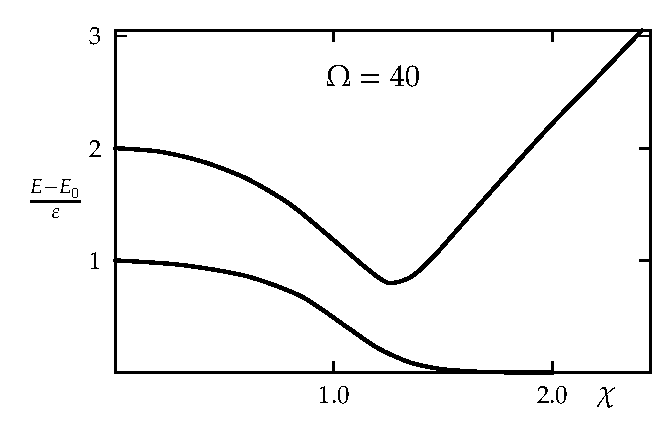
\includegraphics[width=0.75\textwidth]{pictures/10_1}
\par\end{centering}
\caption{\label{fig:10.1}$\Omega=40$ 时第一和第二激发态的激发能量。（引自［Ho 73］。）}
\end{figure}

近似解与精确解无法区分。这并不十分令人惊讶，因为我们知道 GCM 能够产生精确结果（第 10.4 节），并且在该模型中对称动量展开和高斯重叠方法中忽略的项是$\mathcal{O}(1/\Omega)$的。

\subsection{多维情形}

为简便起见，到目前为止我们仅处理了一个生成坐标。在若干坐标$\boldsymbol{a}=(a_{1},\dots,a_{f})$的一般情况下，Kamlah［Ka
73］以及 Onishi 等人［OU 75］对范数重叠核采用了通用高斯拟设：

\begin{equation}
\mathscr{N}(\boldsymbol{a},\boldsymbol{a}')=\mathscr{N}\left(\boldsymbol{q}+\frac{\boldsymbol{s}}{2},\boldsymbol{q}-\frac{\boldsymbol{s}}{2}\right)=\exp\left(-\frac{1}{2}s^{2}(\boldsymbol{q},\boldsymbol{s})\right),\label{eq:10.142}
\end{equation}

其中$\boldsymbol{q}=\frac{1}{2}(\boldsymbol{a}+\boldsymbol{a}'),\boldsymbol{s}=\boldsymbol{a}-\boldsymbol{a}'$，且

\begin{equation}
s^{2}=\gamma_{ij}(\boldsymbol{q})s^{i}s^{j}\label{eq:10.143}
\end{equation}

是由坐标$\boldsymbol{a}$表征的弯曲空间中的测地距离平方。应用 Riemann 空间理论，人们可以如第 10.7.4
节那样推进，并最终得到集体 Hamiltonian：

\begin{equation}
\mathscr{H}_{\mathrm{coll}}=-\frac{1}{\sqrt{\gamma}}\frac{\partial}{\partial q^{i}}\sqrt{\gamma}\left(\frac{\hbar^{2}}{2M}\right)^{ij}\frac{\partial}{\partial q^{j}}+\tilde{V}(\boldsymbol{q}),\label{eq:10.144}
\end{equation}

其中$\gamma(\boldsymbol{q})$是由拟设 (10.143) 定义的度规张量$\gamma_{ik}$的行列式。惯性张量和势具有与式
(10.134) 等类似的形式：

\begin{align}
\left(\frac{\hbar^{2}}{2M(\boldsymbol{q})}\right)_{ij} & =\left.-\frac{1}{4}\left(\frac{\Delta}{\Delta q^{i}}\frac{\Delta}{\Delta q^{j}}h(\boldsymbol{q},\boldsymbol{q}')-\frac{\Delta}{\Delta q^{i}}\frac{\Delta}{\Delta q'^{j}}h(\boldsymbol{q},\boldsymbol{q}')\right)\right|_{\boldsymbol{q}=\boldsymbol{q}'},\nonumber \\
V(\boldsymbol{q}) & =\tilde{V}(\boldsymbol{q})-\epsilon_{0}(\boldsymbol{q});\quad\tilde{V}(\boldsymbol{q})=\langle\boldsymbol{q}|H|\boldsymbol{q}\rangle,\nonumber \\
\epsilon_{0}(\boldsymbol{q}) & =\gamma_{ij}\left(\frac{\hbar^{2}}{2M}\right)^{ij}+\frac{1}{8}\gamma^{ij}\frac{\Delta}{\Delta q^{i}}\frac{\Delta}{\Delta q^{j}}\tilde{V}(\boldsymbol{q}),\label{eq:10.145}
\end{align}

其中$\Delta/\Delta q^{i}$是张量场的协变微商，例如在［LL 59, 卷 II, 第 10 章］中所定义的。动能算符类似于我们从
Pauli 量子化中得到的算符［式 (1.53)］。然而在后一种情况下，惯性张量与度规张量是相同的。现在我们必须区分完全由运动学性质（即由$\mathscr{N}$）决定的度规，与由$\mathscr{H}$的动力学行为给出的惯性。

\section{集体坐标的选取}

在第 10.4 节中我们看到，如果我们选取足够多的生成坐标，拟设 (10.2) 原则上包含了多体问题的精确解答。不幸的是，这是一个大到无法精确处理的问题，在实践中我们每次仅限于处理一个或也许少数几个生成坐标。因此，选取适当的生成坐标——即最合适的集合$|q\rangle=|\Phi(q)\rangle$——是非常重要的。在下文中，我们再次将自己限制在具有时间偶函数$|q\rangle$的实坐标$q$上。

生成函数集$|\Phi(q)\rangle$代表了多维能量曲面

\[
E[\Phi]=\langle\Phi|H|\Phi\rangle
\]

中的一条路径。为了确定这条路径，我们再次应用变分原理，并要求态

\begin{equation}
|\Psi\rangle=\int f(q)|\Phi(q)\rangle\,\mathrm{d}q\label{eq:10.146}
\end{equation}

中的能量期望值不仅关于权重函数$f$的变分是平稳的，而且关于路径$|\Phi(q)\rangle$也是平稳的。这种双重变分方法给出了我们一组耦合方程［HY
74, Vi 75］：

\begin{align}
\int\mathrm{d}q'\,\langle\Phi(q)|H-E|\Phi(q')\rangle f(q') & =0,\label{eq:10.147a}\\
\int\mathrm{d}q\,\mathrm{d}q'\,f^{*}(q)\langle\delta\Phi(q)|H-E|\Phi(q')\rangle f(q') & =0,\label{eq:10.147b}
\end{align}

它们原则上必须通过迭代来求解。

在点$q$处，变分$|\delta\Phi\rangle$并非完全任意。我们只能允许与路径本身正交的改变$|\delta\Phi\rangle_{\perp}$。平行于路径的变分可以被吸收到权重函数的变分中。

由于$|\delta\Phi\rangle_{\perp}$的长度是任意的，式 (10.147b) 可以写为

\begin{equation}
\int\mathrm{d}q'\,\prescript{}{\perp}{\langle}\delta\Phi(q)|H-E|\Phi(q')\rangle f(q')=0.\label{eq:10.148}
\end{equation}

在下一步中，我们做两个基本假定：

(i) 我们再次利用重叠函数$\langle\Phi(q)|\cdots|\Phi(q')\rangle$在$q=q'$处呈现尖锐峰值的事实，使得对于固定的$q$，仅有某个$q'$区域对积分
(10.148) 有贡献。

(ii) 我们假定在这一$q'$区域内，路径弯曲得不太强烈，使得$|\delta\Phi(q)\rangle$在这整个区域内都与路径正交。

在这些条件下，第二个方程 (10.147b) 与第一个方程 (10.147a) 解耦，并且对于不改变$|\Phi\rangle$范数的变分$|\delta\Phi\rangle_{\perp}$［Vi
75］，我们发现：

\begin{equation}
\prescript{}{\perp}{\langle}\delta\Phi|H|\Phi\rangle=0.\label{eq:10.149}
\end{equation}

变分$|\delta\Phi\rangle_{\perp}$受限于与路径正交。平行于路径的变分由下式给出：

\begin{equation}
|\delta\Phi\rangle_{\parallel}=|\Phi(q+\delta q)\rangle-|\Phi(q)\rangle=-\delta q\frac{\mathrm{i}}{\hbar}\hat{P}|\Phi(q)\rangle.\label{eq:10.150}
\end{equation}

算符$\hat{P}$是多体 Hilbert 空间中$-(\hbar/\mathrm{i})\partial/\partial q$的表象。它作用在$|\Phi\rangle$中的粒子坐标上，而不作用在参数$q$上。与路径正交的变分现在具有如下形式：

\begin{equation}
|\delta\Phi\rangle_{\perp}=|\delta\Phi\rangle-\hat{P}|\Phi\rangle\frac{\langle\Phi|\hat{P}|\delta\Phi\rangle}{\langle\Phi|\hat{P}^{2}|\Phi\rangle},\label{eq:10.151}
\end{equation}

其中$|\delta\Phi\rangle$是无限制的变分。势能$V(q)=\langle\Phi(q)|H|\Phi(q)\rangle$平行于路径的变分由下式给出：

\begin{equation}
\frac{\mathrm{d}V}{\mathrm{d}q}=+\frac{\mathrm{i}}{\hbar}\langle\Phi|[\hat{P},H]|\Phi\rangle,\label{eq:10.152}
\end{equation}

而与路径正交的变分必须消失：

\begin{equation}
\prescript{}{\perp}{\langle}\delta\Phi|H|\Phi\rangle=\left\langle \delta\Phi\middle|H-\frac{\hbar}{2\mathrm{i}}\frac{\mathrm{d}V}{\mathrm{d}q}\frac{\hat{P}}{\langle\Phi|\hat{P}^{2}|\Phi\rangle}\middle|\Phi\right\rangle =0.\label{eq:10.153}
\end{equation}

在导出该方程时，我们使用了式 (10.152) 以及$|\Phi\rangle$为时间偶的事实。问题 (10.153) 是一个有约束的变分原理，但约束算符不是
Hermite 的；因此我们将自己限制在$\hat{P}$可以被分解的情形：

\begin{equation}
\hat{P}=\mathrm{i}(A^{\dagger}-A),\quad\text{其中 }A|\Phi\rangle=0.\label{eq:10.154}
\end{equation}

例子是 Slater 行列式$|\Phi(q)\rangle$，此时我们有$A^{\dagger}=(1/\mathrm{i})\sum_{mi}P_{mi}a^{\dagger}_{m}a_{i}$；或者是
RPA 波函数，其中$A^{\dagger}$是玻色子的产生算符（亦参见［ABC 77b］）。

在此类情况下，我们可以定义一个 Hermite 约束算符：

\begin{equation}
\hat{Q}=\frac{\hbar}{2\langle\Phi|\hat{P}^{2}|\Phi\rangle}(A^{\dagger}+A),\label{eq:10.155}
\end{equation}

并由式 (10.152) 和 (10.153) 得到

\begin{equation}
\left\langle \delta\Phi\middle|H-\frac{\mathrm{d}V}{\mathrm{d}q}\cdot\hat{Q}\middle|\Phi\right\rangle =0,\label{eq:10.156}
\end{equation}

这给出了我们最优路径。它以如下方式确定：能量曲面关于垂直于路径的所有变分都具有极小值。这意味着，例如，它沿着裂变谷的底部行进（参见第
7.6 节）。式 (10.156) 是一个带约束的变分问题。约束算符$\hat{Q}$不是强加给系统的，而是由系统本身自洽决定的。它不会将系统推入非物理区域，而是像
d'Alembert 意义下的惯性力一样起作用［Vi 77］。

$|\Phi(q)\rangle$的实际计算需要双重迭代：从约束算符的某个初始值$\hat{Q}_{0}$开始，我们必须通过约束
HF 计算来确定$|\Phi_{0}(q)\rangle$。在第二步中，我们必须在每个点$q$处计算算符$\hat{P}$。例如，这可以通过在线性响应理论中求解式
(8.106) 来完成［参见式 (8.136) 和 (12.120)］。由算符$\hat{P}$可以确定新的约束$\hat{Q}$。这必须持续进行直到实现收敛。

最后，我们必须针对已确定的生成函数$|\Phi(q)\rangle$求解 Hill-Wheeler 方程 (10.5)。

这种双重迭代自然是极其耗时的，在 GCM 中自洽约束的规定迄今仅在三能级 Lipkin 模型［HY 74］以及$s-d$壳［PL
77］中进行了检验，并取得了相当有希望的结果。对于更重的核，第 7 章中描述的梯度方法可以简化该问题。

\section{GCM 在束缚态中的应用}

在过去几年中，GCM 已被应用于核结构的许多问题，例如巨共振、形状振动和对振动，以及核裂变和重离子碰撞（参见第 12 章）。方程 (10.5)
通常通过离散化求解。在许多情况下，只要在数值上消除范数的零本征值，极少数的网格点就已足够。在下文中我们仅讨论少数几个例子。

\subsection{巨共振}

轻核中的呼吸模和四极振荡已使用变形振子函数的 Slater 行列式$\Phi_{JM,P}(b,\beta)$进行了研究，这些基矢被投影到好角动量$J,M$和线动量$P=0$；它们依赖于振子长度$b=(b^{2}_{x}b_{z})^{1/3}$和形变$\beta=b_{x}/b_{z}$［CBA
73, AC 75］。对于$\beta=1$，参数$b$描述了径向坐标的标度变换，因此对应于呼吸模。（Ferrell 和 Visscher
在早期的一篇论文中就已使用过它［FV 56］）。坐标$\beta$描述了四极振荡。Hill-Wheeler 方程 (10.5) 采用
Brink 和 Boeker 相互作用［BB 67］通过离散化（多达 50 个网格点）求解。每个$J$值的最低本征态给出了基态转动带。它与投影
HF 波函数非常吻合。激发态是振动。人们在能谱以及跃迁矩中发现了非简谐性，以及不同模式之间的耦合。

Faessler 等人［KRG 76］以约束 HF 波函数$\Phi(r_{p},r_{n})$作为生成态，研究了满壳核$^{16}\mathrm{O}$、$^{40}\mathrm{Ca}$、$^{90}\mathrm{Zr}$和$^{208}\mathrm{Pb}$中的单极模式。坐标$r_{p},r_{n}$是质子和中子的均方根半径，约束算符（参见第
7 章）由下式给出：

\[
r^{2}\left(1+\exp\left(\frac{r-R}{a}\right)\right)^{-1}.
\]

Fermi 分布确保了约束算符是有界的，相应的 HF Hamiltonian 具有分立本征态。与连续谱的耦合被忽略。相互作用是 Skyrme
类型的修正$\delta$相互作用，在此情况下重叠积分$\mathscr{H}$可以以简单的方式计算。通过约束 HF 计算，标度规定可以得到检验，并发现它是完全合理的。方程
(10.5) 再次通过离散化求解。GCM 的基态能量与 HF 能量非常吻合。激发态是呼吸模。表 10.1 给出了一些结果。

\begin{table}[htbp]
\caption{\label{tab:10.1}呼吸模的 GCM 计算结果：激发能量$E$、约化跃迁几率、能量加权求和规则 (8.154) 的份额$S$、质子和中子跃迁振幅$A_{p}$与$A_{n}$、同位旋期望值$\langle T^{2}\rangle$以及质子和中子半径$r_{p}$与$r_{n}$。（引自［KRG
76］。）}

\centering{}%
\begin{tabular}{ccccccccc}
\toprule 
核素 & $E\,(\mathrm{MeV})$ & $B(E0)\,(\mathrm{fm}^{4})$ & $S$ & $A_{p}\,(\mathrm{fm}^{2})$ & $A_{n}\,(\mathrm{fm}^{2})$ & $\langle T^{2}\rangle$ & $r_{p}\,(\mathrm{fm})$ & $r_{n}\,(\mathrm{fm})$\tabularnewline
\midrule
$^{16}\mathrm{O}$ & 0 &  &  &  &  & 0.00 & 2.70 & 2.67\tabularnewline
 & 23.96 & 106 & 0.56 & 10.3 & 9.7 & 0.00 & 2.91 & 2.86\tabularnewline
$^{40}\mathrm{Ca}$ & 0 &  &  &  &  & 0.02 & 3.41 & 3.36\tabularnewline
 & 20.73 & 502 & 0.55 & 22.4 & 20.4 & 0.14 & 3.50 & 3.44\tabularnewline
$^{90}\mathrm{Zr}$ & 0 &  &  &  &  & 30.12 & 4.22 & 4.30\tabularnewline
 & 17.46 & 1530 & 0.45 & 39.1 & 49.8 & 30.12 & 4.25 & 4.33\tabularnewline
$^{208}\mathrm{Pb}$ & 0 &  &  &  &  & 506.38 & 5.46 & 5.66\tabularnewline
 & 13.32 & 5749 & 0.36 & 75.8 & 127.4 & 506.41 & 5.47 & 5.67\tabularnewline
 & 21.29 & 359 & 0.04 & -19.0 & 130.6 & 506.59 & 5.45 & 5.71\tabularnewline
 & 38.18 & 239 & 0.04 & -15.4 & 26.3 & 506.68 & 5.44 & 5.79\tabularnewline
\bottomrule
\end{tabular}
\end{table}

$^{208}\mathrm{Pb}$中同标呼吸模的能量为 13.32 MeV，与不可压缩性（式 (5.95)）$K\sim200\,\text{MeV}$的液滴模型以及采用
Migdal 力的 RPA 计算［RS 74a］非常吻合。

带有可变振子参数的振子波函数基底中的 Skyrme 相互作用（参见第 4.4.3 节）为$\mathscr{H}$和$\mathscr{N}$提供了相当简单的解析表达式。它们被
Giraud 和 Grammaticos［GG 75］结合矩展开（参见第 10.7 节）用于单极模式的描述。Flocard 和 Vautherin［FV
75, 76］利用振子波函数的 Slater 行列式和 Skyrme 力，通过离散化（多达 143 个网格点）求解了单极、四极和偶极激发的
HW 方程 (10.5)：基态再次与 HF 态非常吻合。图 10.2 显示了$^{16}\mathrm{O}$中基态 ($g_{0}$)
和前两个激发呼吸模 ($g_{1},g_{2}$) 的权重函数$g_{i}$［式 (10.12)］，以及能量重叠核的对角部分（式
(10.135) 中的$\mathscr{H}(r,r)$），它大致对应于集体坐标的势$V(r)$。我们看到函数$g_{i}$在此势中的定性行为类似于振子函数。

\begin{figure}[htbp]
\begin{centering}
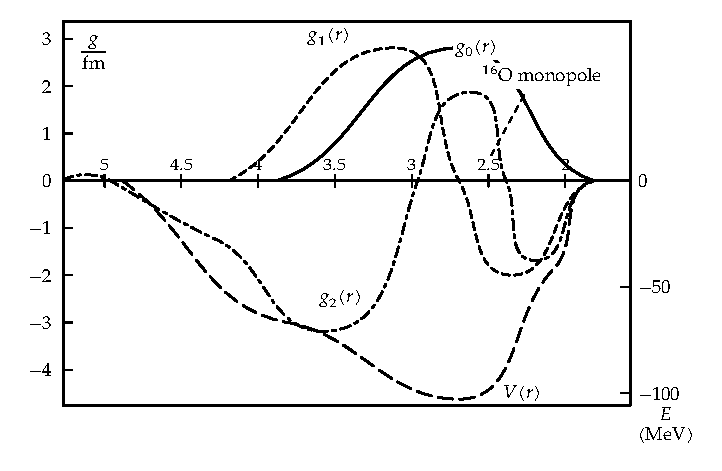
\includegraphics[width=0.75\textwidth]{pictures/10_2}
\par\end{centering}
\caption{\label{fig:10.2}单极振动情形下$^{16}\mathrm{O}$中前三个 GCM 态的权重函数$g_{i}$以及能量重叠核的对角部分$V(r)$。（引自［FV
76］。）}
\end{figure}

随着质量数的增加，函数$g_{0}$的宽度减小。对于重核，它在生成坐标的某个确定值处呈现尖锐的峰值。这意味着 GCM 波函数在很好近似下由带有该参数的
Slater 行列式给出。

GCM 也已被应用于轻核中的低激发形状振动。只要我们将它们限制在仅包含$s\text{-}d$壳的组态空间［GMA 75, MMR
75］，它们就可以与该子空间中 Hamiltonian 的精确对角化［PW 72, Wh 72, SZ 72］进行比较，并且发现许多能级都符合得很好。然而在某些情况下，符合得相当差。这意味着相应的态并不落在由生成函数张成的空间中。纯四极约束［KK
74］的效果此时不如第 10.8 节所讨论的由系统本身决定的约束算符［PL 77］。

\subsection{对振动}

在第 8.8 节中我们看到，在基于正常流体基态的 RPA 对对振动的描述中，对于临界耦合常数$G_{c}$我们发现了相变。在这一区域，RPA
和 BCS 模型都不能很好地工作。GCM 提供了一种克服这一困难的方法。

若干作者［JMR 72, ISY 73］提出使用投影到好粒子数的 BCS 波函数［参见式 (6.31)］（参见第 11.4 节）作为生成态：

\begin{equation}
|\Phi^{N}\rangle=P^{N}\prod_{\alpha,m}\left(u_{\alpha}+v_{\alpha}a^{\dagger}_{\alpha m}a^{\dagger}_{\alpha-m}\right)|-\rangle,\label{eq:10.157}
\end{equation}

其中$P^{N}$是向粒子数$N$的投影算符，而$\alpha=(nlj)$是不同$j$壳的量子数。对于独立参数$p_{\alpha}=u_{\alpha}/v_{\alpha}$，这些态张成了全
Hilbert 空间的高级数等于零（seniority-zero）子空间（参见第 6.2 节和［JMR 69］）。对于仅依赖于一个参数$\Delta$的
BCS 形式 (6.59) 的占据几率$u_{\alpha},v_{\alpha}$，这在很好近似下仍然成立。由于我们期望具有$J^{\pi}=0^{+}$的对振动落在该子空间中（参见第
8.8 节），拟设 (10.157) 对于在 GCM 框架内描述它们特别有用。第二个参数，即化学势$\lambda$，可以通过每个$\Delta$网格点处的
BCS 粒子数方程 (6.53) 来确定，或者可以作为第二个生成坐标使用（Sorensen 等人［SS 72b］）。

该方法对于超导核、非超导核以及过渡区域同样有效。它已被采用纯配对力［SS 72b, FGP 73］应用于简单模型以及 Pb、Ni 和
Sn 区域中的对振动能谱。

图 10.3 显示了$^{208}\mathrm{Pb}$基态以及 4.87 MeV 处所谓的对振动态的 GCM 波函数组分，后者在很大程度上是一个$2p\text{-}2h$态，或者是$^{210}\mathrm{Pb}$中$2p$对振动与$^{206}\mathrm{Pb}$中$2h$对振动的叠加。$0p\text{-}0h$、$2p\text{-}2h$和$4p\text{-}4h$组分作为配对强度$G$的函数给出。给出正确质量差$M(^{206}\mathrm{Pb})+M(^{210}\mathrm{Pb})-2M(^{208}\mathrm{Pb})$的$G$的真实值为$G=0.1166\,\text{MeV}$。在此取值下，基态已经有
10\% 是$2p\text{-}2h$态，而对振动大致有 12\% 的$4p\text{-}4h$掺杂。

\begin{figure}[htbp]
\begin{centering}
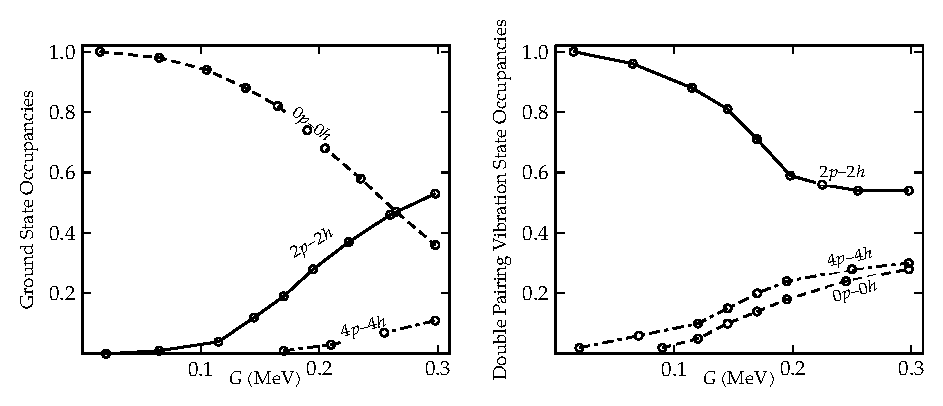
\includegraphics[width=0.85\textwidth]{pictures/10_3}
\par\end{centering}
\caption{\label{fig:10.3}$^{208}\mathrm{Pb}$基态与 4.87 MeV 处对振动态中$0p\text{-}0h$、$2p\text{-}2h$和$4p\text{-}4h$组分百分比随$G$的变化关系。（引自［SS
72b］。）}
\end{figure}

更逼真的核力已被 Faessler 等人［AGM 74］在$p\text{-}f$壳中使用。在此，式 (10.157) 中的 BCS
函数被约束 HFB 函数替换（参见第 7.6 节）。约束算符是可变强度的配对势，生成坐标是由此产生的能量贡献$-\frac{1}{2}\operatorname{Tr}(\kappa^{\dagger}\Delta\kappa)$。生成函数通过向好粒子数和角动量投影从这些
HFB 函数确定。结果与实验能级和转移截面符合良好。

该方法提供了一个研究基态和对振动态中配对关联（通过能隙$\Delta$衡量）对有效配对强度$G_{\mathrm{eff}}$的依赖关系的工具（图
10.4）。在基态强烈配对（大$G_{\mathrm{eff}}$）的情况下，对振动具有微弱的配对关联。例如在稀土核中就是如此。对于基态配对微弱的原子核，如
Ti，情况正好相反（亦参见［Kl 70］）。从第 7.7 节我们知道，Coriolis 反配对效应 (CAP) 随着角动量的增加降低了有效配对强度。这在稀土核的基态中产生降低的配对关联，并在对振动模式中产生增加的配对关联。然而对于较轻的核（如
Ti），这不再成立。

\begin{figure}[htbp]
\begin{centering}
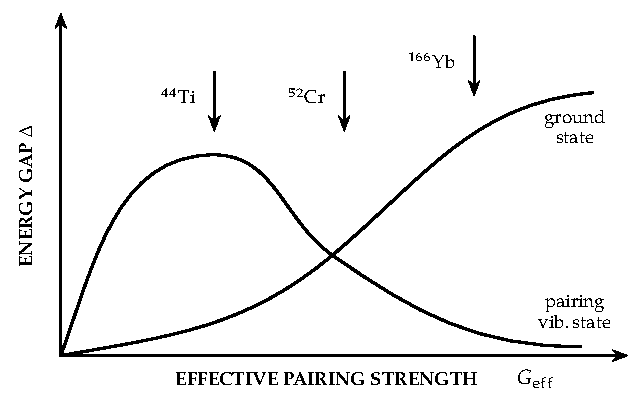
\includegraphics[width=0.75\textwidth]{pictures/10_4}
\par\end{centering}
\caption{\label{fig:10.4}能隙$\Delta$对有效配对强度$G_{\mathrm{eff}}$依赖关系的示意图。箭头指出了若干原子核的位置。（引自［GSF
75］。）}
\end{figure}

最后，如果我们引入更多的生成坐标，如形变参数$\beta$、配对参数$\Delta$等等［MAG 75］，我们可以通过 GCM
描述不同模式之间的各种耦合。我们甚至可以通过做出如下推广拟设来包含单粒子自由度［DMG 76, MGA 77］：

\begin{equation}
|\Psi\rangle=\int\mathrm{d}a\,f(a)|\Phi(a)\rangle+\sum_{i}\int\mathrm{d}a\,f^{i}(a)|\Phi_{i}(a)\rangle,\label{eq:10.158}
\end{equation}

其中$|\Phi(a)\rangle$例如是依赖于某个形变参数$a$的约束 HF 计算的基态，而$|\Phi_{i}(a)\rangle$是相应的$1p\text{-}1h$态，等等。
